\documentclass[a4paper]{book}
\usepackage{a4wide}
\usepackage{makeidx}
\usepackage{fancyhdr}
\usepackage{graphicx}
\usepackage{multicol}
\usepackage{float}
\usepackage{textcomp}
\usepackage{alltt}
\usepackage{doxygen}
\makeindex
\setcounter{tocdepth}{1}
\renewcommand{\footrulewidth}{0.4pt}
\begin{document}
\begin{titlepage}
\vspace*{7cm}
\begin{center}
{\Large PARADISEO-MO Reference Manual\\[1ex]\large 0.1 }\\
\vspace*{1cm}
{\large Generated by Doxygen 1.4.7}\\
\vspace*{0.5cm}
{\small Thu Jul 5 17:08:27 2007}\\
\end{center}
\end{titlepage}
\clearemptydoublepage
\pagenumbering{roman}
\tableofcontents
\clearemptydoublepage
\pagenumbering{arabic}
\chapter{Welcome to PARADISEO-Moving Objects }
\label{index}\section{intro}\label{main_intro}
MO is an extension of the ANSI-C++ compliant evolutionary computation library {\bf EO}. \par
 It contains classes for almost any kind of one solution based heuristics.\section{tutorial}\label{main_tutorial}
\section{install}\label{main_install}
The installation procedure of the package is detailed in the {\tt README} file in the top-directory of the source-tree.\section{design}\label{main_design}

\chapter{PARADISEO-MO Hierarchical Index}
\section{Paradis\-EO-MO-Moving\-Objects Class Hierarchy}
This inheritance list is sorted roughly, but not completely, alphabetically:\begin{CompactList}
\item eo\-Functor\-Base{\tt  [external]}\begin{CompactList}
\item eo\-BF$<$ const EOT \&, const EOT \&, bool $>${\tt  [external]}\begin{CompactList}
\item \contentsline{section}{mo\-Comparator$<$ EOT $>$}{\pageref{classmo_comparator}}{}
\begin{CompactList}
\item \contentsline{section}{mo\-Fit\-Comparator$<$ EOT $>$}{\pageref{classmo_fit_comparator}}{}
\end{CompactList}
\end{CompactList}
\item eo\-BF$<$ const M \&, const M::EOType \&, bool $>${\tt  [external]}\begin{CompactList}
\item \contentsline{section}{mo\-Tabu\-List$<$ M $>$}{\pageref{classmo_tabu_list}}{}
\begin{CompactList}
\item \contentsline{section}{mo\-Simple\-Move\-Tabu\-List$<$ M $>$}{\pageref{classmo_simple_move_tabu_list}}{}
\item \contentsline{section}{mo\-Simple\-Solution\-Tabu\-List$<$ M $>$}{\pageref{classmo_simple_solution_tabu_list}}{}
\end{CompactList}
\end{CompactList}
\item eo\-BF$<$ const M \&, const M::EOType \&, M::EOType::Fitness $>${\tt  [external]}\begin{CompactList}
\item \contentsline{section}{mo\-Move\-Incr\-Eval$<$ M $>$}{\pageref{classmo_move_incr_eval}}{}
\end{CompactList}
\item eo\-BF$<$ const M \&, const M::EOType \&, void $>${\tt  [external]}\begin{CompactList}
\item \contentsline{section}{mo\-LSCheck\-Point$<$ M $>$}{\pageref{classmo_l_s_check_point}}{}
\end{CompactList}
\item eo\-BF$<$ const M \&, const M::EOType::Fitness \&, bool $>${\tt  [external]}\begin{CompactList}
\item \contentsline{section}{mo\-Aspir\-Crit$<$ M $>$}{\pageref{classmo_aspir_crit}}{}
\begin{CompactList}
\item \contentsline{section}{mo\-Impr\-Best\-Fit\-Aspir\-Crit$<$ M $>$}{\pageref{classmo_impr_best_fit_aspir_crit}}{}
\item \contentsline{section}{mo\-No\-Aspir\-Crit$<$ M $>$}{\pageref{classmo_no_aspir_crit}}{}
\end{CompactList}
\end{CompactList}
\item eo\-BF$<$ const M::EOType \&, M::EOType \&, void $>${\tt  [external]}\begin{CompactList}
\item \contentsline{section}{mo\-Move\-Expl$<$ M $>$}{\pageref{classmo_move_expl}}{}
\begin{CompactList}
\item \contentsline{section}{mo\-Move\-Loop\-Expl$<$ M $>$}{\pageref{classmo_move_loop_expl}}{}
\begin{CompactList}
\item \contentsline{section}{mo\-HCMove\-Loop\-Expl$<$ M $>$}{\pageref{classmo_h_c_move_loop_expl}}{}
\item \contentsline{section}{mo\-TSMove\-Loop\-Expl$<$ M $>$}{\pageref{classmo_t_s_move_loop_expl}}{}
\end{CompactList}
\end{CompactList}
\end{CompactList}
\item eo\-BF$<$ M \&, const M::EOType \&, bool $>${\tt  [external]}\begin{CompactList}
\item \contentsline{section}{mo\-Next\-Move$<$ M $>$}{\pageref{classmo_next_move}}{}
\begin{CompactList}
\item \contentsline{section}{mo\-It\-Rand\-Next\-Move$<$ M $>$}{\pageref{classmo_it_rand_next_move}}{}
\end{CompactList}
\end{CompactList}
\item eo\-BF$<$ M \&, const M::EOType \&, void $>${\tt  [external]}\begin{CompactList}
\item \contentsline{section}{mo\-Move\-Init$<$ M $>$}{\pageref{classmo_move_init}}{}
\end{CompactList}
\item eo\-BF$<$ M \&, M::EOType::Fitness \&, void $>${\tt  [external]}\begin{CompactList}
\item \contentsline{section}{mo\-Move\-Select$<$ M $>$}{\pageref{classmo_move_select}}{}
\begin{CompactList}
\item \contentsline{section}{mo\-Best\-Impr\-Select$<$ M $>$}{\pageref{classmo_best_impr_select}}{}
\item \contentsline{section}{mo\-First\-Impr\-Select$<$ M $>$}{\pageref{classmo_first_impr_select}}{}
\item \contentsline{section}{mo\-Rand\-Impr\-Select$<$ M $>$}{\pageref{classmo_rand_impr_select}}{}
\end{CompactList}
\end{CompactList}
\item eo\-UF$<$ const EOT \&, bool $>${\tt  [external]}\begin{CompactList}
\item \contentsline{section}{mo\-Sol\-Continue$<$ EOT $>$}{\pageref{classmo_sol_continue}}{}
\begin{CompactList}
\item \contentsline{section}{mo\-Fit\-Sol\-Continue$<$ EOT $>$}{\pageref{classmo_fit_sol_continue}}{}
\item \contentsline{section}{mo\-Gen\-Sol\-Continue$<$ EOT $>$}{\pageref{classmo_gen_sol_continue}}{}
\item \contentsline{section}{mo\-No\-Fit\-Impr\-Sol\-Continue$<$ EOT $>$}{\pageref{classmo_no_fit_impr_sol_continue}}{}
\item \contentsline{section}{mo\-Steady\-Fit\-Sol\-Continue$<$ EOT $>$}{\pageref{classmo_steady_fit_sol_continue}}{}
\end{CompactList}
\end{CompactList}
\item eo\-UF$<$ double \&, bool $>${\tt  [external]}\begin{CompactList}
\item \contentsline{section}{mo\-Cooling\-Schedule}{\pageref{classmo_cooling_schedule}}{}
\begin{CompactList}
\item \contentsline{section}{mo\-Exponential\-Cooling\-Schedule}{\pageref{classmo_exponential_cooling_schedule}}{}
\item \contentsline{section}{mo\-Linear\-Cooling\-Schedule}{\pageref{classmo_linear_cooling_schedule}}{}
\end{CompactList}
\end{CompactList}
\item eo\-UF$<$ EOT \&, bool $>${\tt  [external]}\begin{CompactList}
\item eo\-Mon\-Op$<$ EOT $>${\tt  [external]}\begin{CompactList}
\item \contentsline{section}{mo\-Algo$<$ EOT $>$}{\pageref{classmo_algo}}{}
\end{CompactList}
\end{CompactList}
\item eo\-UF$<$ EOT \&, void $>${\tt  [external]}\begin{CompactList}
\item \contentsline{section}{mo\-Move$<$ EOT $>$}{\pageref{classmo_move}}{}
\end{CompactList}
\item eo\-UF$<$ EOType \&, bool $>${\tt  [external]}\item eo\-UF$<$ M \&, void $>${\tt  [external]}\begin{CompactList}
\item \contentsline{section}{mo\-Rand\-Move$<$ M $>$}{\pageref{classmo_rand_move}}{}
\end{CompactList}
\item eo\-UF$<$ M::EOType \&, bool $>${\tt  [external]}\begin{CompactList}
\item eo\-Mon\-Op$<$ M::EOType $>${\tt  [external]}\begin{CompactList}
\item \contentsline{section}{mo\-Algo$<$ M::EOType $>$}{\pageref{classmo_algo}}{}
\begin{CompactList}
\item \contentsline{section}{mo\-HC$<$ M $>$}{\pageref{classmo_h_c}}{}
\item \contentsline{section}{mo\-ILS$<$ M $>$}{\pageref{classmo_i_l_s}}{}
\item \contentsline{section}{mo\-SA$<$ M $>$}{\pageref{classmo_s_a}}{}
\item \contentsline{section}{mo\-TS$<$ M $>$}{\pageref{classmo_t_s}}{}
\end{CompactList}
\end{CompactList}
\end{CompactList}
\end{CompactList}
\item eo\-Op$<$ EOType $>${\tt  [external]}\begin{CompactList}
\item eo\-Mon\-Op$<$ EOT $>${\tt  [external]}\item eo\-Mon\-Op$<$ M::EOType $>${\tt  [external]}\end{CompactList}
\end{CompactList}

\chapter{PARADISEO-MO Class Index}
\section{ParadisEO-MOMovingObjects Class List}
Here are the classes, structs, unions and interfaces with brief descriptions:\begin{CompactList}
\item\contentsline{section}{{\bf EmptySelection} (Special class that describes the case of no selection )}{\pageref{class_empty_selection}}{}
\item\contentsline{section}{{\bf moAlgo$<$ EOT $>$} (Description of an algorithm of the paradiseo-mo library )}{\pageref{classmo_algo}}{}
\item\contentsline{section}{{\bf moAspirCrit$<$ M $>$} (Description of the conditions in which a tabu move could be accepted )}{\pageref{classmo_aspir_crit}}{}
\item\contentsline{section}{{\bf moBestImprSelect$<$ M $>$} (One of the possible \doxyref{moMoveSelect}{p.}{classmo_move_select} )}{\pageref{classmo_best_impr_select}}{}
\item\contentsline{section}{{\bf moComparator$<$ EOT $>$} (Template for classes which need to compare two EOT and indicate if the first is \char`\"{}better\char`\"{} than the second )}{\pageref{classmo_comparator}}{}
\item\contentsline{section}{{\bf moCoolingSchedule} (This class gives the description of a cooling schedule )}{\pageref{classmo_cooling_schedule}}{}
\item\contentsline{section}{{\bf moExponentialCoolingSchedule} (One of the possible \doxyref{moCoolingSchedule}{p.}{classmo_cooling_schedule} )}{\pageref{classmo_exponential_cooling_schedule}}{}
\item\contentsline{section}{{\bf moFirstImprSelect$<$ M $>$} (One possible \doxyref{moMoveSelect}{p.}{classmo_move_select} )}{\pageref{classmo_first_impr_select}}{}
\item\contentsline{section}{{\bf moFitComparator$<$ EOT $>$} (Comparison according to the fitness )}{\pageref{classmo_fit_comparator}}{}
\item\contentsline{section}{{\bf moFitSolContinue$<$ EOT $>$} (One possible stop criterion for a solution-based heuristic )}{\pageref{classmo_fit_sol_continue}}{}
\item\contentsline{section}{{\bf moGenSolContinue$<$ EOT $>$} (One possible stop criterion for a solution-based heuristic )}{\pageref{classmo_gen_sol_continue}}{}
\item\contentsline{section}{{\bf moHC$<$ M $>$} (Hill Climbing (HC) )}{\pageref{classmo_h_c}}{}
\item\contentsline{section}{{\bf moHCMoveLoopExpl$<$ M $>$} (Iterative explorer used by a \doxyref{moHC}{p.}{classmo_h_c} )}{\pageref{classmo_h_c_move_loop_expl}}{}
\item\contentsline{section}{{\bf moILS$<$ M $>$} (Iterated Local Search (ILS) )}{\pageref{classmo_i_l_s}}{}
\item\contentsline{section}{{\bf moImprBestFitAspirCrit$<$ M $>$} (One of the possible \doxyref{moAspirCrit}{p.}{classmo_aspir_crit} )}{\pageref{classmo_impr_best_fit_aspir_crit}}{}
\item\contentsline{section}{{\bf moItRandNextMove$<$ M $>$} (One of the possible \doxyref{moNextMove}{p.}{classmo_next_move} )}{\pageref{classmo_it_rand_next_move}}{}
\item\contentsline{section}{{\bf moLinearCoolingSchedule} (One of the possible \doxyref{moCoolingSchedule}{p.}{classmo_cooling_schedule} )}{\pageref{classmo_linear_cooling_schedule}}{}
\item\contentsline{section}{{\bf moLSCheckPoint$<$ M $>$} (Class which allows a checkpointing system )}{\pageref{classmo_l_s_check_point}}{}
\item\contentsline{section}{{\bf moMove$<$ EOT $>$} (Definition of a move )}{\pageref{classmo_move}}{}
\item\contentsline{section}{{\bf moMoveExpl$<$ M $>$} (Description of a move (\doxyref{moMove}{p.}{classmo_move}) explorer )}{\pageref{classmo_move_expl}}{}
\item\contentsline{section}{{\bf moMoveIncrEval$<$ M $>$} ((generally) Efficient evaluation function based a move and a solution )}{\pageref{classmo_move_incr_eval}}{}
\item\contentsline{section}{{\bf moMoveInit$<$ M $>$} (Move (\doxyref{moMove}{p.}{classmo_move}) initializer )}{\pageref{classmo_move_init}}{}
\item\contentsline{section}{{\bf moMoveLoopExpl$<$ M $>$} (Class which describes an iterative explorer )}{\pageref{classmo_move_loop_expl}}{}
\item\contentsline{section}{{\bf moMoveSelect$<$ M $>$} (Class that describes a move selector (\doxyref{moMove}{p.}{classmo_move}) )}{\pageref{classmo_move_select}}{}
\item\contentsline{section}{{\bf moNextMove$<$ M $>$} (Class which allows to generate a new move (\doxyref{moMove}{p.}{classmo_move}) )}{\pageref{classmo_next_move}}{}
\item\contentsline{section}{{\bf moNoAspirCrit$<$ M $>$} (One of the possible aspiration criterion (\doxyref{moAspirCrit}{p.}{classmo_aspir_crit}) )}{\pageref{classmo_no_aspir_crit}}{}
\item\contentsline{section}{{\bf moNoFitImprSolContinue$<$ EOT $>$} (One possible stop criterion for a solution-based heuristic )}{\pageref{classmo_no_fit_impr_sol_continue}}{}
\item\contentsline{section}{{\bf moRandImprSelect$<$ M $>$} (One of the possible \doxyref{moMove}{p.}{classmo_move} selector (\doxyref{moMoveSelect}{p.}{classmo_move_select}) )}{\pageref{classmo_rand_impr_select}}{}
\item\contentsline{section}{{\bf moRandMove$<$ M $>$} (Random move generator )}{\pageref{classmo_rand_move}}{}
\item\contentsline{section}{{\bf moSA$<$ M $>$} (Simulated Annealing (SA) )}{\pageref{classmo_s_a}}{}
\item\contentsline{section}{{\bf moSimpleMoveTabuList$<$ M $>$} (Class describing a move tabu list with a limited memory )}{\pageref{classmo_simple_move_tabu_list}}{}
\item\contentsline{section}{{\bf moSimpleSolutionTabuList$<$ M $>$} (Class describing a solution tabu list with limited length )}{\pageref{classmo_simple_solution_tabu_list}}{}
\item\contentsline{section}{{\bf moSolContinue$<$ EOT $>$} (Class that describes a stop criterion for a solution-based heuristic )}{\pageref{classmo_sol_continue}}{}
\item\contentsline{section}{{\bf moSteadyFitSolContinue$<$ EOT $>$} (One possible stopping criterion for a solution-based heuristic )}{\pageref{classmo_steady_fit_sol_continue}}{}
\item\contentsline{section}{{\bf moTabuList$<$ M $>$} (Class describing a tabu list that a \doxyref{moTS}{p.}{classmo_t_s} uses )}{\pageref{classmo_tabu_list}}{}
\item\contentsline{section}{{\bf moTS$<$ M $>$} (Tabu Search (TS) )}{\pageref{classmo_t_s}}{}
\item\contentsline{section}{{\bf moTSMoveLoopExpl$<$ M $>$} (Explorer for a Tabu Search algorithm )}{\pageref{classmo_t_s_move_loop_expl}}{}
\end{CompactList}

\chapter{PARADISEO-MO Class Documentation}
\section{EmptySelection Class Reference}
\label{class_empty_selection}\index{EmptySelection@{EmptySelection}}
Special class that describes the case of no selection.  


{\tt \#include $<$moMoveSelect.h$>$}



\subsection{Detailed Description}
Special class that describes the case of no selection. 

This class is used as an exception that can be thrown if a solution selector has completly failed. 



Definition at line 21 of file moMoveSelect.h.

The documentation for this class was generated from the following file:\begin{CompactItemize}
\item 
moMoveSelect.h\end{CompactItemize}

\section{mo\-Algo$<$ EOT $>$ Class Template Reference}
\label{classmo_algo}\index{moAlgo@{moAlgo}}
Description of an algorithm of the paradiseo-mo library.  


{\tt \#include $<$mo\-Algo.h$>$}

Inheritance diagram for mo\-Algo$<$ EOT $>$::\begin{figure}[H]
\begin{center}
\leavevmode
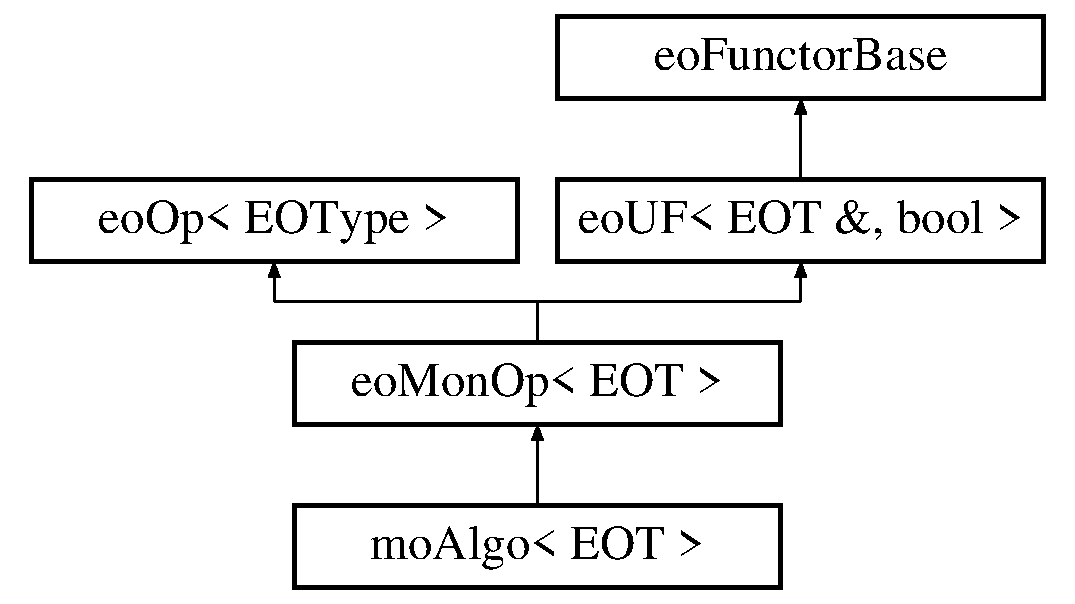
\includegraphics[height=4cm]{classmo_algo}
\end{center}
\end{figure}


\subsection{Detailed Description}
\subsubsection*{template$<$class EOT$>$ class mo\-Algo$<$ EOT $>$}

Description of an algorithm of the paradiseo-mo library. 

{\bf mo\-HC}{\rm (p.\,\pageref{classmo_h_c})}, {\bf mo\-TS}{\rm (p.\,\pageref{classmo_t_s})} and {\bf mo\-SA}{\rm (p.\,\pageref{classmo_s_a})} are 3 examples of algorithm of the paradiseo-mo library. 



Definition at line 46 of file mo\-Algo.h.

The documentation for this class was generated from the following file:\begin{CompactItemize}
\item 
mo\-Algo.h\end{CompactItemize}

\section{mo\-Aspir\-Crit$<$ M $>$ Class Template Reference}
\label{classmo_aspir_crit}\index{moAspirCrit@{moAspirCrit}}
Description of the conditions in which a tabu move could be accepted.  


{\tt \#include $<$mo\-Aspir\-Crit.h$>$}

Inheritance diagram for mo\-Aspir\-Crit$<$ M $>$::\begin{figure}[H]
\begin{center}
\leavevmode
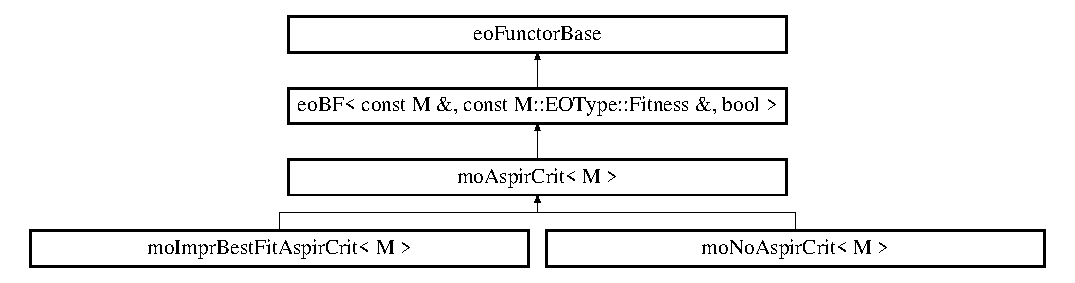
\includegraphics[height=4cm]{classmo_aspir_crit}
\end{center}
\end{figure}
\subsection*{Public Member Functions}
\begin{CompactItemize}
\item 
virtual void \bf{init} ()=0
\begin{CompactList}\small\item\em Procedure which initialises all that needs an aspiration criterion. \item\end{CompactList}\end{CompactItemize}


\subsection{Detailed Description}
\subsubsection*{template$<$class M$>$ class mo\-Aspir\-Crit$<$ M $>$}

Description of the conditions in which a tabu move could be accepted. 

It is only a description... An object that herits from this class is needed to be used in a \doxyref{mo\-TS}{p.}{classmo_t_s}. See mo\-No\-Aspri\-Crit for example. 



Definition at line 47 of file mo\-Aspir\-Crit.h.

\subsection{Member Function Documentation}
\index{moAspirCrit@{mo\-Aspir\-Crit}!init@{init}}
\index{init@{init}!moAspirCrit@{mo\-Aspir\-Crit}}
\subsubsection{\setlength{\rightskip}{0pt plus 5cm}template$<$class M$>$ virtual void \bf{mo\-Aspir\-Crit}$<$ M $>$::init ()\hspace{0.3cm}{\tt  [pure virtual]}}\label{classmo_aspir_crit_a8ce84510a5ec7c9078381e542c6d140}


Procedure which initialises all that needs an aspiration criterion. 

It can be possible that this procedure does nothing... 

Implemented in \bf{mo\-Impr\-Best\-Fit\-Aspir\-Crit$<$ M $>$} \doxyref{p.}{classmo_impr_best_fit_aspir_crit_ffa451a14ff4ea86fb8bd9fdbc348630}, and \bf{mo\-No\-Aspir\-Crit$<$ M $>$} \doxyref{p.}{classmo_no_aspir_crit_f3a286fc4c2d36bd390ba9a3074f3037}.

The documentation for this class was generated from the following file:\begin{CompactItemize}
\item 
mo\-Aspir\-Crit.h\end{CompactItemize}

\section{mo\-Best\-Impr\-Select$<$ M $>$ Class Template Reference}
\label{classmo_best_impr_select}\index{moBestImprSelect@{moBestImprSelect}}
One of the possible {\bf mo\-Move\-Select}{\rm (p.\,\pageref{classmo_move_select})}.  


{\tt \#include $<$mo\-Best\-Impr\-Select.h$>$}

Inheritance diagram for mo\-Best\-Impr\-Select$<$ M $>$::\begin{figure}[H]
\begin{center}
\leavevmode
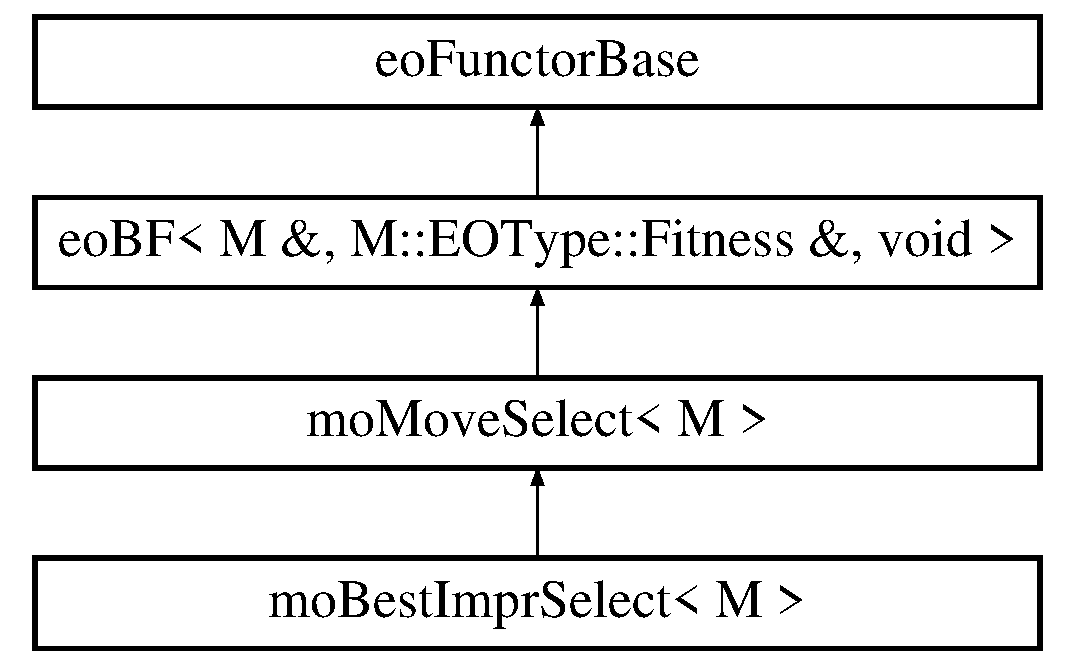
\includegraphics[height=4cm]{classmo_best_impr_select}
\end{center}
\end{figure}
\subsection*{Public Types}
\begin{CompactItemize}
\item 
typedef M::EOType::Fitness {\bf Fitness}\label{classmo_best_impr_select_w0}

\begin{CompactList}\small\item\em Alias for the fitness. \item\end{CompactList}\end{CompactItemize}
\subsection*{Public Member Functions}
\begin{CompactItemize}
\item 
void {\bf init} (const {\bf Fitness} \&\_\-fitness)
\begin{CompactList}\small\item\em Procedure which initialise the exploration. \item\end{CompactList}\item 
bool {\bf update} (const M \&\_\-move, const {\bf Fitness} \&\_\-fitness)
\begin{CompactList}\small\item\em Function that indicates if the current move has not improved the fitness. \item\end{CompactList}\item 
void {\bf operator()} (M \&\_\-move, {\bf Fitness} \&\_\-fitness)
\begin{CompactList}\small\item\em Procedure which saved the best move and fitness. \item\end{CompactList}\end{CompactItemize}
\subsection*{Private Attributes}
\begin{CompactItemize}
\item 
bool {\bf first\_\-time}\label{classmo_best_impr_select_r0}

\begin{CompactList}\small\item\em Allowing to know if at least one move has been generated. \item\end{CompactList}\item 
M {\bf best\_\-move}\label{classmo_best_impr_select_r1}

\begin{CompactList}\small\item\em The best move. \item\end{CompactList}\item 
{\bf Fitness} {\bf best\_\-fitness}\label{classmo_best_impr_select_r2}

\begin{CompactList}\small\item\em The best fitness. \item\end{CompactList}\end{CompactItemize}


\subsection{Detailed Description}
\subsubsection*{template$<$class M$>$ class mo\-Best\-Impr\-Select$<$ M $>$}

One of the possible {\bf mo\-Move\-Select}{\rm (p.\,\pageref{classmo_move_select})}. 

All neighbors are considered, and the movement which enables the best improvement is selected. 



Definition at line 47 of file mo\-Best\-Impr\-Select.h.

\subsection{Member Function Documentation}
\index{moBestImprSelect@{mo\-Best\-Impr\-Select}!init@{init}}
\index{init@{init}!moBestImprSelect@{mo\-Best\-Impr\-Select}}
\subsubsection{\setlength{\rightskip}{0pt plus 5cm}template$<$class M$>$ void {\bf mo\-Best\-Impr\-Select}$<$ M $>$::init (const {\bf Fitness} \& {\em \_\-fitness})\hspace{0.3cm}{\tt  [inline, virtual]}}\label{classmo_best_impr_select_a0}


Procedure which initialise the exploration. 

\begin{Desc}
\item[Parameters:]
\begin{description}
\item[{\em \_\-fitness}]The current fitness. \end{description}
\end{Desc}


Implements {\bf mo\-Move\-Select$<$ M $>$} {\rm (p.\,\pageref{classmo_move_select_a0})}.

Definition at line 58 of file mo\-Best\-Impr\-Select.h.

References mo\-Best\-Impr\-Select$<$ M $>$::first\_\-time, and mo\-Best\-Impr\-Select$<$ M $>$::Fitness.\index{moBestImprSelect@{mo\-Best\-Impr\-Select}!update@{update}}
\index{update@{update}!moBestImprSelect@{mo\-Best\-Impr\-Select}}
\subsubsection{\setlength{\rightskip}{0pt plus 5cm}template$<$class M$>$ bool {\bf mo\-Best\-Impr\-Select}$<$ M $>$::update (const M \& {\em \_\-move}, const {\bf Fitness} \& {\em \_\-fitness})\hspace{0.3cm}{\tt  [inline, virtual]}}\label{classmo_best_impr_select_a1}


Function that indicates if the current move has not improved the fitness. 

If the given fitness enables an improvment, the move ({\bf mo\-Move}{\rm (p.\,\pageref{classmo_move})}) and the fitness linked to this move are saved.

\begin{Desc}
\item[Parameters:]
\begin{description}
\item[{\em \_\-move}]a move. \item[{\em \_\-fitness}]a fitness linked to the move. \end{description}
\end{Desc}
\begin{Desc}
\item[Returns:]TRUE if the move does not improve the fitness. \end{Desc}


Implements {\bf mo\-Move\-Select$<$ M $>$} {\rm (p.\,\pageref{classmo_move_select_a1})}.

Definition at line 77 of file mo\-Best\-Impr\-Select.h.

References mo\-Best\-Impr\-Select$<$ M $>$::best\_\-fitness, mo\-Best\-Impr\-Select$<$ M $>$::best\_\-move, and mo\-Best\-Impr\-Select$<$ M $>$::first\_\-time.\index{moBestImprSelect@{mo\-Best\-Impr\-Select}!operator()@{operator()}}
\index{operator()@{operator()}!moBestImprSelect@{mo\-Best\-Impr\-Select}}
\subsubsection{\setlength{\rightskip}{0pt plus 5cm}template$<$class M$>$ void {\bf mo\-Best\-Impr\-Select}$<$ M $>$::operator() (M \& {\em \_\-move}, {\bf Fitness} \& {\em \_\-fitness})\hspace{0.3cm}{\tt  [inline]}}\label{classmo_best_impr_select_a2}


Procedure which saved the best move and fitness. 

\begin{Desc}
\item[Parameters:]
\begin{description}
\item[{\em \_\-move}]the current move (result of the procedure). \item[{\em \_\-fitness}]the current fitness (result of the procedure). \end{description}
\end{Desc}


Definition at line 95 of file mo\-Best\-Impr\-Select.h.

The documentation for this class was generated from the following file:\begin{CompactItemize}
\item 
mo\-Best\-Impr\-Select.h\end{CompactItemize}

\section{moCoolingSchedule Class Reference}
\label{classmo_cooling_schedule}\index{moCoolingSchedule@{moCoolingSchedule}}
This class gives the description of a cooling schedule.  


{\tt \#include $<$moCoolingSchedule.h$>$}

Inheritance diagram for moCoolingSchedule::\begin{figure}[H]
\begin{center}
\leavevmode
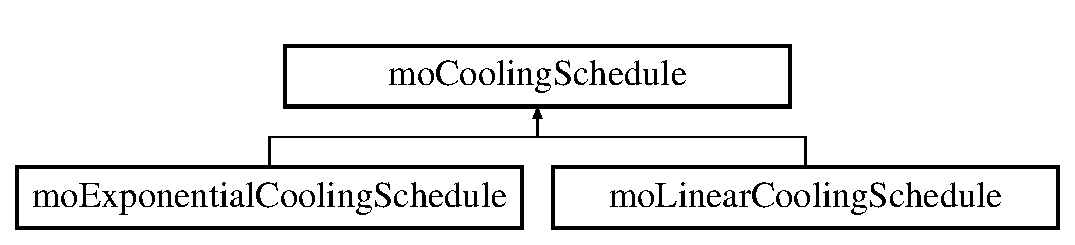
\includegraphics[height=2cm]{classmo_cooling_schedule}
\end{center}
\end{figure}


\subsection{Detailed Description}
This class gives the description of a cooling schedule. 

It is only a description... An object that herits from this class is needed to be used in a \doxyref{moSA}{p.}{classmo_s_a}. See \doxyref{moExponentialCoolingSchedule}{p.}{classmo_exponential_cooling_schedule} or \doxyref{moLinearCoolingSchedule}{p.}{classmo_linear_cooling_schedule} for example. 



Definition at line 22 of file moCoolingSchedule.h.

The documentation for this class was generated from the following file:\begin{CompactItemize}
\item 
moCoolingSchedule.h\end{CompactItemize}

\section{moExponentialCoolingSchedule Class Reference}
\label{classmo_exponential_cooling_schedule}\index{moExponentialCoolingSchedule@{moExponentialCoolingSchedule}}
One of the possible \doxyref{moCoolingSchedule}{p.}{classmo_cooling_schedule}.  


{\tt \#include $<$moExponentialCoolingSchedule.h$>$}

Inheritance diagram for moExponentialCoolingSchedule::\begin{figure}[H]
\begin{center}
\leavevmode
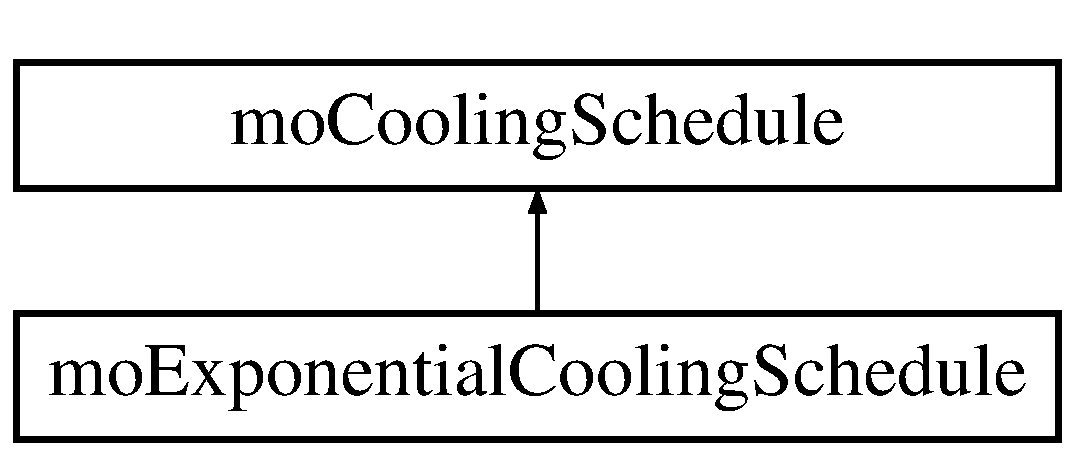
\includegraphics[height=4cm]{classmo_exponential_cooling_schedule}
\end{center}
\end{figure}
\subsection*{Public Member Functions}
\begin{CompactItemize}
\item 
{\bf moExponentialCoolingSchedule} (double \_\-\_\-threshold, double \_\-\_\-ratio)
\begin{CompactList}\small\item\em Simple constructor. \item\end{CompactList}\item 
bool {\bf operator()} (double \&\_\-\_\-temp)
\begin{CompactList}\small\item\em {\bf Function} which proceeds to the cooling. \item\end{CompactList}\end{CompactItemize}
\subsection*{Private Attributes}
\begin{CompactItemize}
\item 
double {\bf threshold}\label{classmo_exponential_cooling_schedule_8d4327c0bb33b7121a322279eea97f84}

\begin{CompactList}\small\item\em The temperature threhold. \item\end{CompactList}\item 
double {\bf ratio}\label{classmo_exponential_cooling_schedule_e8f3f87417c1c7253efb938a740846fa}

\begin{CompactList}\small\item\em The decreasing factor of the temperature. \item\end{CompactList}\end{CompactItemize}


\subsection{Detailed Description}
One of the possible \doxyref{moCoolingSchedule}{p.}{classmo_cooling_schedule}. 

An other very simple cooling schedule, the temperature decrease according to a ratio while the temperature is greater than a given threshold. 



Definition at line 45 of file moExponentialCoolingSchedule.h.

\subsection{Constructor \& Destructor Documentation}
\index{moExponentialCoolingSchedule@{moExponentialCoolingSchedule}!moExponentialCoolingSchedule@{moExponentialCoolingSchedule}}
\index{moExponentialCoolingSchedule@{moExponentialCoolingSchedule}!moExponentialCoolingSchedule@{moExponentialCoolingSchedule}}
\subsubsection{\setlength{\rightskip}{0pt plus 5cm}moExponentialCoolingSchedule::moExponentialCoolingSchedule (double {\em \_\-\_\-threshold}, double {\em \_\-\_\-ratio})\hspace{0.3cm}{\tt  [inline]}}\label{classmo_exponential_cooling_schedule_b01930c1051c0940666c6325bfd036bc}


Simple constructor. 

\begin{Desc}
\item[Parameters:]
\begin{description}
\item[{\em \_\-\_\-threshold}]the threshold. \item[{\em \_\-\_\-ratio}]the ratio used to descrease the temperature. \end{description}
\end{Desc}


Definition at line 54 of file moExponentialCoolingSchedule.h.

\subsection{Member Function Documentation}
\index{moExponentialCoolingSchedule@{moExponentialCoolingSchedule}!operator()@{operator()}}
\index{operator()@{operator()}!moExponentialCoolingSchedule@{moExponentialCoolingSchedule}}
\subsubsection{\setlength{\rightskip}{0pt plus 5cm}bool moExponentialCoolingSchedule::operator() (double \& {\em \_\-\_\-temp})\hspace{0.3cm}{\tt  [inline, virtual]}}\label{classmo_exponential_cooling_schedule_00642b03453b51612a10fcf2280543db}


{\bf Function} which proceeds to the cooling. 

It decreases the temperature and indicates if it is greater than the threshold.

\begin{Desc}
\item[Parameters:]
\begin{description}
\item[{\em \_\-\_\-temp}]the current temperature. \end{description}
\end{Desc}
\begin{Desc}
\item[Returns:]if the new temperature (current temperature $\ast$ ratio) is greater than the threshold. \end{Desc}


Implements {\bf eoUF$<$ double \&, bool $>$}.

Definition at line 64 of file moExponentialCoolingSchedule.h.

References ratio, and threshold.

The documentation for this class was generated from the following file:\begin{CompactItemize}
\item 
moExponentialCoolingSchedule.h\end{CompactItemize}

\section{mo\-First\-Impr\-Select$<$ M $>$ Class Template Reference}
\label{classmo_first_impr_select}\index{moFirstImprSelect@{moFirstImprSelect}}
One possible \doxyref{mo\-Move\-Select}{p.}{classmo_move_select}.  


{\tt \#include $<$mo\-First\-Impr\-Select.h$>$}

Inheritance diagram for mo\-First\-Impr\-Select$<$ M $>$::\begin{figure}[H]
\begin{center}
\leavevmode
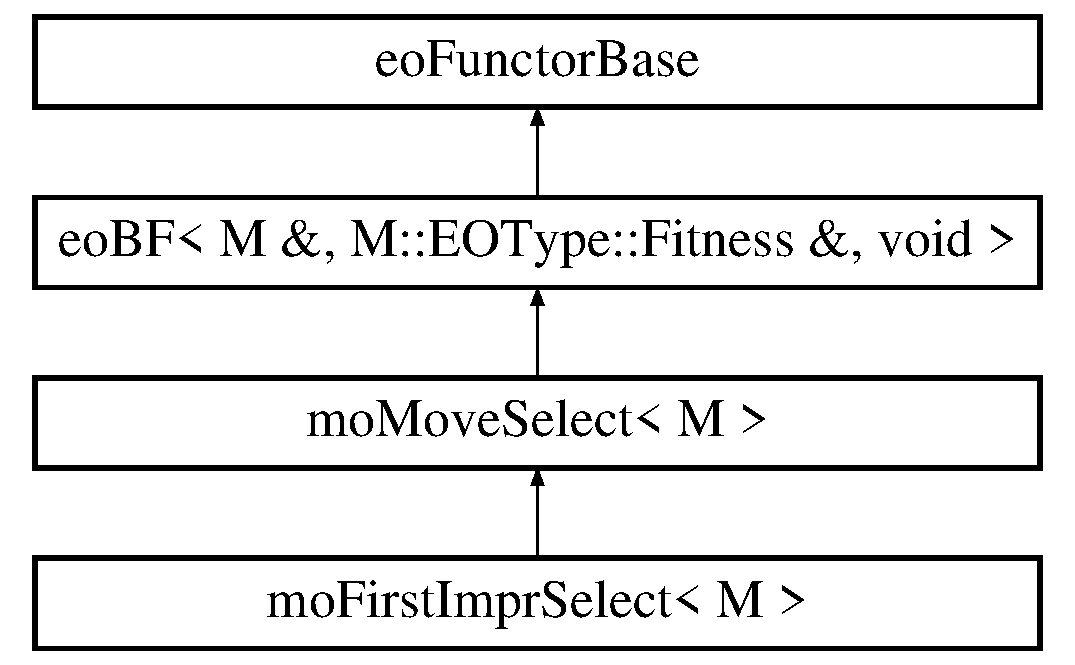
\includegraphics[height=2cm]{classmo_first_impr_select}
\end{center}
\end{figure}
\subsection*{Public Types}
\begin{CompactItemize}
\item 
typedef M::EOType::Fitness \bf{Fitness}\label{classmo_first_impr_select_64763ce3e6d2873266624382b407fa5a}

\begin{CompactList}\small\item\em Alias for the fitness. \item\end{CompactList}\end{CompactItemize}
\subsection*{Public Member Functions}
\begin{CompactItemize}
\item 
virtual void \bf{init} (const \bf{Fitness} \&\_\-\_\-fit)
\begin{CompactList}\small\item\em Procedure which initialise the exploration. \item\end{CompactList}\item 
bool \bf{update} (const M \&\_\-\_\-move, const typename M::EOType::Fitness \&\_\-\_\-fit)
\begin{CompactList}\small\item\em Function that indicates if the current move has not improved the fitness. \item\end{CompactList}\item 
void \bf{operator()} (M \&\_\-\_\-move, \bf{Fitness} \&\_\-\_\-fit)  throw (Empty\-Selection)
\begin{CompactList}\small\item\em Procedure which saved the best move and fitness. \item\end{CompactList}\end{CompactItemize}
\subsection*{Private Attributes}
\begin{CompactItemize}
\item 
bool \bf{valid}\label{classmo_first_impr_select_a99c0586ba07449234705c17a258d58c}

\begin{CompactList}\small\item\em Allow to know if at least one move has improved the solution. \item\end{CompactList}\item 
M \bf{best\_\-move}\label{classmo_first_impr_select_dfed419a608dd7c41f07fa1f1279cb8c}

\begin{CompactList}\small\item\em Best stored movement. \item\end{CompactList}\item 
\bf{Fitness} \bf{init\_\-fit}\label{classmo_first_impr_select_ce7ba63e8cc3a9164f4e546477e98ca8}

\begin{CompactList}\small\item\em Initial fitness. \item\end{CompactList}\item 
\bf{Fitness} \bf{best\_\-fit}\label{classmo_first_impr_select_e1190347b76ec6fe717be32354b4a9a9}

\begin{CompactList}\small\item\em Best stored fitness. \item\end{CompactList}\end{CompactItemize}


\subsection{Detailed Description}
\subsubsection*{template$<$class M$>$ class mo\-First\-Impr\-Select$<$ M $>$}

One possible \doxyref{mo\-Move\-Select}{p.}{classmo_move_select}. 

The neighborhood is explored until a move enables an improvement of the current solution. 



Definition at line 23 of file mo\-First\-Impr\-Select.h.

\subsection{Member Function Documentation}
\index{moFirstImprSelect@{mo\-First\-Impr\-Select}!init@{init}}
\index{init@{init}!moFirstImprSelect@{mo\-First\-Impr\-Select}}
\subsubsection{\setlength{\rightskip}{0pt plus 5cm}template$<$class M$>$ virtual void \bf{mo\-First\-Impr\-Select}$<$ M $>$::init (const \bf{Fitness} \& {\em \_\-\_\-fit})\hspace{0.3cm}{\tt  [inline, virtual]}}\label{classmo_first_impr_select_4c5ce18ede46247a439c68f6954a4055}


Procedure which initialise the exploration. 

It save the current fitness as the initial value for the fitness. 

Implements \bf{mo\-Move\-Select$<$ M $>$} \doxyref{p.}{classmo_move_select_bca4c43f13d26eca7163aeb272a4a52e}.

Definition at line 35 of file mo\-First\-Impr\-Select.h.

References mo\-First\-Impr\-Select$<$ M $>$::init\_\-fit, and mo\-First\-Impr\-Select$<$ M $>$::valid.\index{moFirstImprSelect@{mo\-First\-Impr\-Select}!update@{update}}
\index{update@{update}!moFirstImprSelect@{mo\-First\-Impr\-Select}}
\subsubsection{\setlength{\rightskip}{0pt plus 5cm}template$<$class M$>$ bool \bf{mo\-First\-Impr\-Select}$<$ M $>$::update (const M \& {\em \_\-\_\-move}, const typename M::EOType::Fitness \& {\em \_\-\_\-fit})\hspace{0.3cm}{\tt  [inline]}}\label{classmo_first_impr_select_7ba0882728daedc75c249647c070ccf0}


Function that indicates if the current move has not improved the fitness. 

If the given fitness enables an improvement, the move (\doxyref{mo\-Move}{p.}{classmo_move}) should be applied to the current solution.

\begin{Desc}
\item[Parameters:]
\begin{description}
\item[{\em \_\-\_\-move}]a move. \item[{\em \_\-\_\-fit}]a fitness linked to the move. \end{description}
\end{Desc}
\begin{Desc}
\item[Returns:]TRUE if the move does not improve the fitness. \end{Desc}


Definition at line 52 of file mo\-First\-Impr\-Select.h.

References mo\-First\-Impr\-Select$<$ M $>$::best\_\-fit, mo\-First\-Impr\-Select$<$ M $>$::best\_\-move, mo\-First\-Impr\-Select$<$ M $>$::init\_\-fit, and mo\-First\-Impr\-Select$<$ M $>$::valid.\index{moFirstImprSelect@{mo\-First\-Impr\-Select}!operator()@{operator()}}
\index{operator()@{operator()}!moFirstImprSelect@{mo\-First\-Impr\-Select}}
\subsubsection{\setlength{\rightskip}{0pt plus 5cm}template$<$class M$>$ void \bf{mo\-First\-Impr\-Select}$<$ M $>$::operator() (M \& {\em \_\-\_\-move}, \bf{Fitness} \& {\em \_\-\_\-fit})  throw (\bf{Empty\-Selection})\hspace{0.3cm}{\tt  [inline]}}\label{classmo_first_impr_select_3be12cf4cbaed00df7c4fa735b2c0a95}


Procedure which saved the best move and fitness. 

\begin{Desc}
\item[Parameters:]
\begin{description}
\item[{\em \_\-\_\-move}]the current move (result of the procedure). \item[{\em \_\-\_\-fit}]the current fitness (result of the procedure). \end{description}
\end{Desc}
\begin{Desc}
\item[Exceptions:]
\begin{description}
\item[{\em \doxyref{Empty\-Selection}{p.}{class_empty_selection}}]if no move has improved the fitness. \end{description}
\end{Desc}


Definition at line 76 of file mo\-First\-Impr\-Select.h.

References mo\-First\-Impr\-Select$<$ M $>$::best\_\-fit, mo\-First\-Impr\-Select$<$ M $>$::best\_\-move, and mo\-First\-Impr\-Select$<$ M $>$::valid.

The documentation for this class was generated from the following file:\begin{CompactItemize}
\item 
mo\-First\-Impr\-Select.h\end{CompactItemize}

\section{mo\-Gen\-Sol\-Continue$<$ EOT $>$ Class Template Reference}
\label{classmo_gen_sol_continue}\index{moGenSolContinue@{moGenSolContinue}}
One possible stop criterion for a solution-based heuristic.  


{\tt \#include $<$mo\-Gen\-Sol\-Continue.h$>$}

Inheritance diagram for mo\-Gen\-Sol\-Continue$<$ EOT $>$::\begin{figure}[H]
\begin{center}
\leavevmode
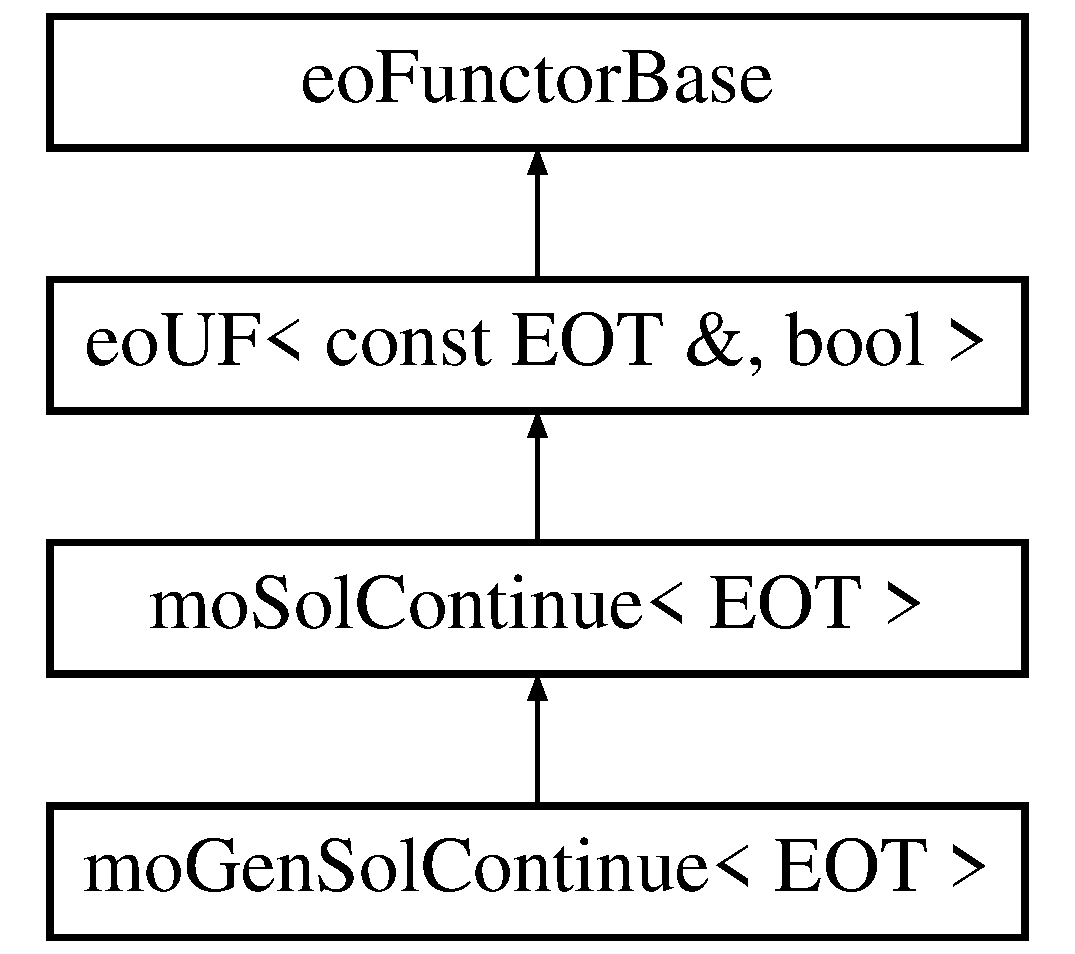
\includegraphics[height=4cm]{classmo_gen_sol_continue}
\end{center}
\end{figure}
\subsection*{Public Member Functions}
\begin{CompactItemize}
\item 
\bf{mo\-Gen\-Sol\-Continue} (unsigned int \_\-\_\-max\-Num\-Gen)
\begin{CompactList}\small\item\em Simple constructor. \item\end{CompactList}\item 
bool \bf{operator()} (const EOT \&\_\-\_\-sol)
\begin{CompactList}\small\item\em \doxyref{Function} that activates the stop criterion. \item\end{CompactList}\item 
void \bf{init} ()
\begin{CompactList}\small\item\em Procedure which allows to initialise the generation counter. \item\end{CompactList}\end{CompactItemize}
\subsection*{Private Attributes}
\begin{CompactItemize}
\item 
unsigned int \bf{max\-Num\-Gen}\label{classmo_gen_sol_continue_30b9861e090578bdfa2374806600987a}

\begin{CompactList}\small\item\em Iteration maximum number. \item\end{CompactList}\item 
unsigned int \bf{num\-Gen}\label{classmo_gen_sol_continue_630d9736a3a2c952540cdc211764258c}

\begin{CompactList}\small\item\em Iteration current number. \item\end{CompactList}\end{CompactItemize}


\subsection{Detailed Description}
\subsubsection*{template$<$class EOT$>$ class mo\-Gen\-Sol\-Continue$<$ EOT $>$}

One possible stop criterion for a solution-based heuristic. 

The stop criterion corresponds to a maximum number of iteration. 



Definition at line 46 of file mo\-Gen\-Sol\-Continue.h.

\subsection{Constructor \& Destructor Documentation}
\index{moGenSolContinue@{mo\-Gen\-Sol\-Continue}!moGenSolContinue@{moGenSolContinue}}
\index{moGenSolContinue@{moGenSolContinue}!moGenSolContinue@{mo\-Gen\-Sol\-Continue}}
\subsubsection{\setlength{\rightskip}{0pt plus 5cm}template$<$class EOT$>$ \bf{mo\-Gen\-Sol\-Continue}$<$ EOT $>$::\bf{mo\-Gen\-Sol\-Continue} (unsigned int {\em \_\-\_\-max\-Num\-Gen})\hspace{0.3cm}{\tt  [inline]}}\label{classmo_gen_sol_continue_b56e890f1caa3f98e161c6512b59c95b}


Simple constructor. 

\begin{Desc}
\item[Parameters:]
\begin{description}
\item[{\em \_\-\_\-max\-Num\-Gen}]the maximum number of generation. \end{description}
\end{Desc}


Definition at line 55 of file mo\-Gen\-Sol\-Continue.h.

\subsection{Member Function Documentation}
\index{moGenSolContinue@{mo\-Gen\-Sol\-Continue}!operator()@{operator()}}
\index{operator()@{operator()}!moGenSolContinue@{mo\-Gen\-Sol\-Continue}}
\subsubsection{\setlength{\rightskip}{0pt plus 5cm}template$<$class EOT$>$ bool \bf{mo\-Gen\-Sol\-Continue}$<$ EOT $>$::operator() (const EOT \& {\em \_\-\_\-sol})\hspace{0.3cm}{\tt  [inline, virtual]}}\label{classmo_gen_sol_continue_457257cd73b474d6f7783d84d02c2e61}


\doxyref{Function} that activates the stop criterion. 

Increments the counter and returns TRUE if the current number of iteration is lower than the given maximum number of iterations.

\begin{Desc}
\item[Parameters:]
\begin{description}
\item[{\em \_\-\_\-sol}]the current solution. \end{description}
\end{Desc}
\begin{Desc}
\item[Returns:]TRUE or FALSE according to the current generation number. \end{Desc}


Implements \bf{eo\-UF$<$ const EOT \&, bool $>$}.

Definition at line 69 of file mo\-Gen\-Sol\-Continue.h.

References mo\-Gen\-Sol\-Continue$<$ EOT $>$::max\-Num\-Gen, and mo\-Gen\-Sol\-Continue$<$ EOT $>$::num\-Gen.\index{moGenSolContinue@{mo\-Gen\-Sol\-Continue}!init@{init}}
\index{init@{init}!moGenSolContinue@{mo\-Gen\-Sol\-Continue}}
\subsubsection{\setlength{\rightskip}{0pt plus 5cm}template$<$class EOT$>$ void \bf{mo\-Gen\-Sol\-Continue}$<$ EOT $>$::init ()\hspace{0.3cm}{\tt  [inline, virtual]}}\label{classmo_gen_sol_continue_6c5db8182157584b56507cc9075602d4}


Procedure which allows to initialise the generation counter. 

It can also be used to reset the iteration counter. 

Implements \bf{mo\-Sol\-Continue$<$ EOT $>$} \doxyref{p.}{classmo_sol_continue_064dc966a210f4ffb9515be3f03ca4c7}.

Definition at line 79 of file mo\-Gen\-Sol\-Continue.h.

References mo\-Gen\-Sol\-Continue$<$ EOT $>$::num\-Gen.

The documentation for this class was generated from the following file:\begin{CompactItemize}
\item 
mo\-Gen\-Sol\-Continue.h\end{CompactItemize}

\section{mo\-HC$<$ M $>$ Class Template Reference}
\label{classmo_h_c}\index{moHC@{moHC}}
Hill Climbing (HC).  


{\tt \#include $<$mo\-HC.h$>$}

Inheritance diagram for mo\-HC$<$ M $>$::\begin{figure}[H]
\begin{center}
\leavevmode
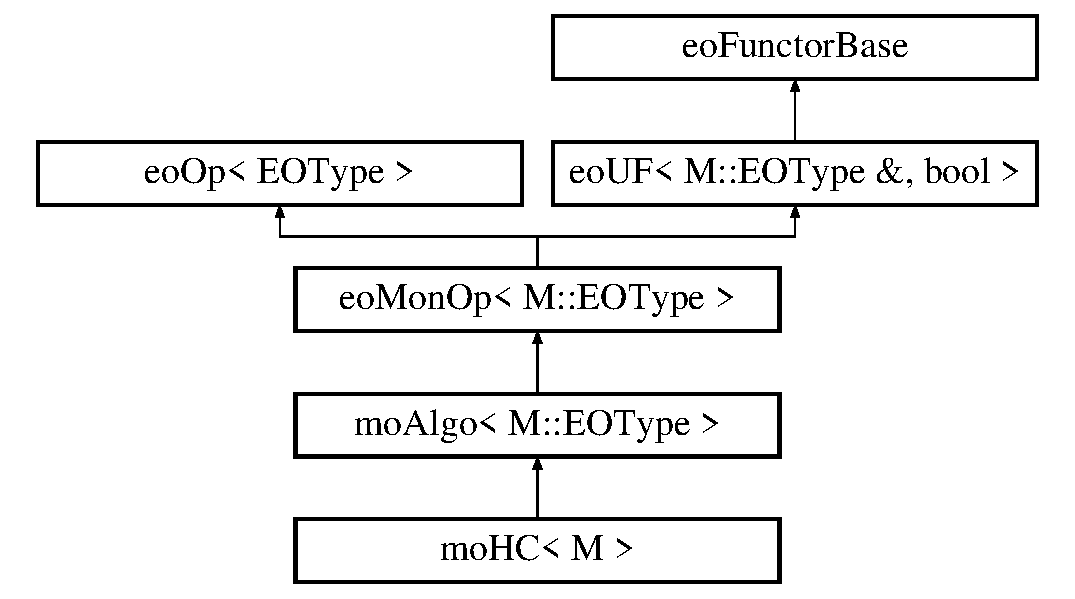
\includegraphics[height=5cm]{classmo_h_c}
\end{center}
\end{figure}
\subsection*{Public Member Functions}
\begin{CompactItemize}
\item 
\bf{mo\-HC} (\bf{mo\-Move\-Init}$<$ M $>$ \&\_\-\_\-move\_\-init, \bf{mo\-Next\-Move}$<$ M $>$ \&\_\-\_\-next\_\-move, \bf{mo\-Move\-Incr\-Eval}$<$ M $>$ \&\_\-\_\-incr\_\-eval, \bf{mo\-Move\-Select}$<$ M $>$ \&\_\-\_\-move\_\-select, \bf{eo\-Eval\-Func}$<$ \bf{EOT} $>$ \&\_\-\_\-full\_\-eval)
\begin{CompactList}\small\item\em Full constructor. \item\end{CompactList}\item 
\bf{mo\-HC} (\bf{mo\-Move\-Expl}$<$ M $>$ \&\_\-\_\-move\_\-expl, \bf{eo\-Eval\-Func}$<$ \bf{EOT} $>$ \&\_\-\_\-full\_\-eval)
\begin{CompactList}\small\item\em Light constructor. \item\end{CompactList}\item 
bool \bf{operator()} (\bf{EOT} \&\_\-\_\-sol)
\begin{CompactList}\small\item\em \doxyref{Function} which launches the HC. \item\end{CompactList}\end{CompactItemize}
\subsection*{Private Types}
\begin{CompactItemize}
\item 
typedef M::EOType \bf{EOT}\label{classmo_h_c_d219296ede03c679646bce2fe8ff96cb}

\begin{CompactList}\small\item\em Alias for the type. \item\end{CompactList}\item 
typedef EOT::Fitness \bf{Fitness}\label{classmo_h_c_56487c97a7cf0c423cc879d1bbd45027}

\begin{CompactList}\small\item\em Alias for the fitness. \item\end{CompactList}\end{CompactItemize}
\subsection*{Private Attributes}
\begin{CompactItemize}
\item 
\bf{mo\-Move\-Expl}$<$ M $>$ \& \bf{move\_\-expl}\label{classmo_h_c_f6bfb4553fb699f1e08f7d9c37d06103}

\begin{CompactList}\small\item\em Complete exploration of the neighborhood. \item\end{CompactList}\item 
\bf{eo\-Eval\-Func}$<$ \bf{EOT} $>$ \& \bf{full\_\-eval}\label{classmo_h_c_4b0d5cc70fc3d83f59a48b2bdea65736}

\begin{CompactList}\small\item\em A full evaluation function. \item\end{CompactList}\end{CompactItemize}


\subsection{Detailed Description}
\subsubsection*{template$<$class M$>$ class mo\-HC$<$ M $>$}

Hill Climbing (HC). 

Class which describes the algorithm for a hill climbing. 



Definition at line 50 of file mo\-HC.h.

\subsection{Constructor \& Destructor Documentation}
\index{moHC@{mo\-HC}!moHC@{moHC}}
\index{moHC@{moHC}!moHC@{mo\-HC}}
\subsubsection{\setlength{\rightskip}{0pt plus 5cm}template$<$class M$>$ \bf{mo\-HC}$<$ M $>$::\bf{mo\-HC} (\bf{mo\-Move\-Init}$<$ M $>$ \& {\em \_\-\_\-move\_\-init}, \bf{mo\-Next\-Move}$<$ M $>$ \& {\em \_\-\_\-next\_\-move}, \bf{mo\-Move\-Incr\-Eval}$<$ M $>$ \& {\em \_\-\_\-incr\_\-eval}, \bf{mo\-Move\-Select}$<$ M $>$ \& {\em \_\-\_\-move\_\-select}, \bf{eo\-Eval\-Func}$<$ \bf{EOT} $>$ \& {\em \_\-\_\-full\_\-eval})\hspace{0.3cm}{\tt  [inline]}}\label{classmo_h_c_6cafe093f86a80c225827884cb9dc5b7}


Full constructor. 

All the boxes are given in order the HC to use a \doxyref{mo\-HCMove\-Loop\-Expl}{p.}{classmo_h_c_move_loop_expl}.

\begin{Desc}
\item[Parameters:]
\begin{description}
\item[{\em \_\-\_\-move\_\-init}]a move initialiser. \item[{\em \_\-\_\-next\_\-move}]a neighborhood explorer. \item[{\em \_\-\_\-incr\_\-eval}]a (generally) efficient evaluation function. \item[{\em \_\-\_\-move\_\-select}]a move selector. \item[{\em \_\-\_\-full\_\-eval}]a full evaluation function. \end{description}
\end{Desc}


Definition at line 77 of file mo\-HC.h.\index{moHC@{mo\-HC}!moHC@{moHC}}
\index{moHC@{moHC}!moHC@{mo\-HC}}
\subsubsection{\setlength{\rightskip}{0pt plus 5cm}template$<$class M$>$ \bf{mo\-HC}$<$ M $>$::\bf{mo\-HC} (\bf{mo\-Move\-Expl}$<$ M $>$ \& {\em \_\-\_\-move\_\-expl}, \bf{eo\-Eval\-Func}$<$ \bf{EOT} $>$ \& {\em \_\-\_\-full\_\-eval})\hspace{0.3cm}{\tt  [inline]}}\label{classmo_h_c_45f27309792e584a27fa6dcb86ccda65}


Light constructor. 

This constructor allow to use another \doxyref{mo\-Move\-Expl}{p.}{classmo_move_expl} (generally not a \doxyref{mo\-HCMove\-Loop\-Expl}{p.}{classmo_h_c_move_loop_expl}).

\begin{Desc}
\item[Parameters:]
\begin{description}
\item[{\em \_\-\_\-move\_\-expl}]a complete explorer. \item[{\em \_\-\_\-full\_\-eval}]a full evaluation function. \end{description}
\end{Desc}


Definition at line 91 of file mo\-HC.h.

\subsection{Member Function Documentation}
\index{moHC@{mo\-HC}!operator()@{operator()}}
\index{operator()@{operator()}!moHC@{mo\-HC}}
\subsubsection{\setlength{\rightskip}{0pt plus 5cm}template$<$class M$>$ bool \bf{mo\-HC}$<$ M $>$::operator() (\bf{EOT} \& {\em \_\-\_\-sol})\hspace{0.3cm}{\tt  [inline, virtual]}}\label{classmo_h_c_ed4e273c420efa6386c5975a696a5010}


\doxyref{Function} which launches the HC. 

The HC has to improve a current solution. As the \doxyref{mo\-SA}{p.}{classmo_s_a} and the mo TS, it can be used for HYBRIDATION in an evolutionnary algorithm.

\begin{Desc}
\item[Parameters:]
\begin{description}
\item[{\em \_\-\_\-sol}]a current solution to improve. \end{description}
\end{Desc}
\begin{Desc}
\item[Returns:]TRUE. \end{Desc}


Implements \bf{eo\-UF$<$ M::EOType \&, bool $>$}.

Definition at line 106 of file mo\-HC.h.

References mo\-HC$<$ M $>$::full\_\-eval, and mo\-HC$<$ M $>$::move\_\-expl.

The documentation for this class was generated from the following file:\begin{CompactItemize}
\item 
mo\-HC.h\end{CompactItemize}

\section{moHCMoveLoopExpl$<$ M $>$ Class Template Reference}
\label{classmo_h_c_move_loop_expl}\index{moHCMoveLoopExpl@{moHCMoveLoopExpl}}
Iterative explorer used by a \doxyref{moHC}{p.}{classmo_h_c}.  


{\tt \#include $<$moHCMoveLoopExpl.h$>$}

Inheritance diagram for moHCMoveLoopExpl$<$ M $>$::\begin{figure}[H]
\begin{center}
\leavevmode
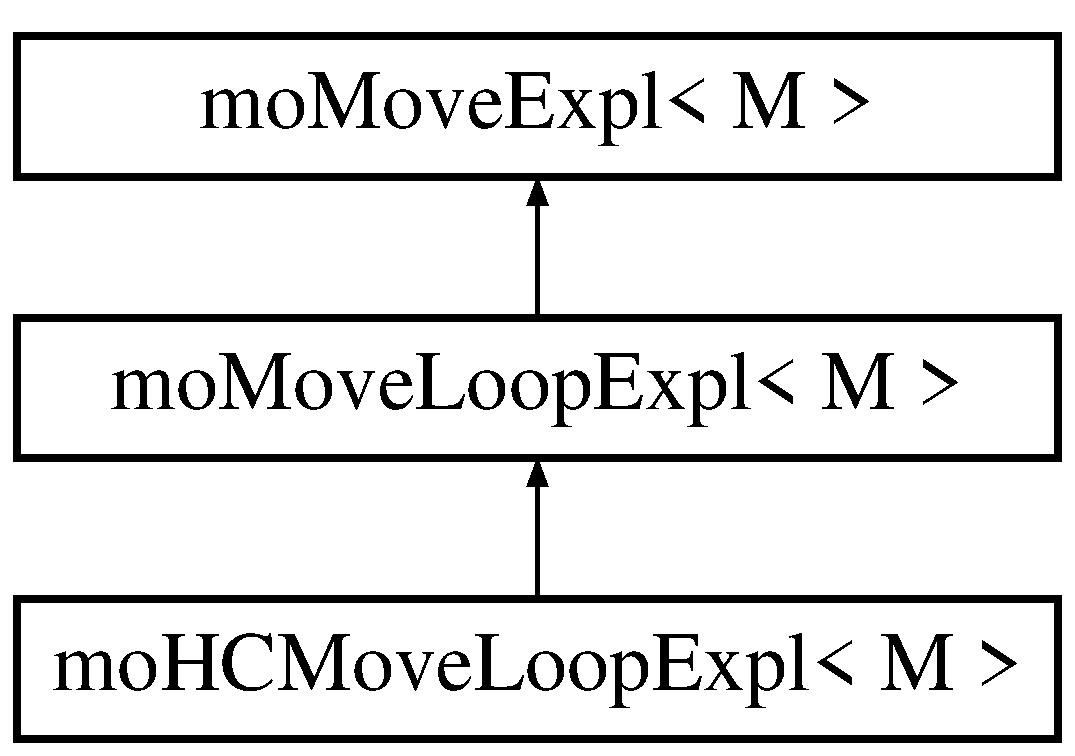
\includegraphics[height=5cm]{classmo_h_c_move_loop_expl}
\end{center}
\end{figure}
\subsection*{Public Member Functions}
\begin{CompactItemize}
\item 
{\bf moHCMoveLoopExpl} ({\bf moMoveInit}$<$ M $>$ \&\_\-\_\-move\_\-init, {\bf moNextMove}$<$ M $>$ \&\_\-\_\-next\_\-move, {\bf moMoveIncrEval}$<$ M $>$ \&\_\-\_\-incr\_\-eval, {\bf moMoveSelect}$<$ M $>$ \&\_\-\_\-move\_\-select)
\begin{CompactList}\small\item\em Constructor. \item\end{CompactList}\item 
void {\bf operator()} (const {\bf EOT} \&\_\-\_\-old\_\-sol, {\bf EOT} \&\_\-\_\-new\_\-sol)
\begin{CompactList}\small\item\em Procedure which launches the explorer. \item\end{CompactList}\end{CompactItemize}
\subsection*{Private Types}
\begin{CompactItemize}
\item 
typedef M::EOType {\bf EOT}\label{classmo_h_c_move_loop_expl_077befd4106c201eafd3ea22bcea2fe9}

\begin{CompactList}\small\item\em Alias for the type. \item\end{CompactList}\item 
typedef M::EOType::Fitness {\bf Fitness}\label{classmo_h_c_move_loop_expl_f24871224316d5549b9013a2d27ab465}

\begin{CompactList}\small\item\em Alias for the fitness. \item\end{CompactList}\end{CompactItemize}
\subsection*{Private Attributes}
\begin{CompactItemize}
\item 
{\bf moMoveInit}$<$ M $>$ \& {\bf move\_\-init}\label{classmo_h_c_move_loop_expl_6776fc51331c1b452d026b92448b4ffc}

\begin{CompactList}\small\item\em Move initialiser. \item\end{CompactList}\item 
{\bf moNextMove}$<$ M $>$ \& {\bf next\_\-move}\label{classmo_h_c_move_loop_expl_f716c5271e0eba9275c585dc52768443}

\begin{CompactList}\small\item\em Neighborhood explorer. \item\end{CompactList}\item 
{\bf moMoveIncrEval}$<$ M $>$ \& {\bf incr\_\-eval}\label{classmo_h_c_move_loop_expl_84a8fccba05ab30414281469bc8ee779}

\begin{CompactList}\small\item\em (generally) Efficient evaluation. \item\end{CompactList}\item 
{\bf moMoveSelect}$<$ M $>$ \& {\bf move\_\-select}\label{classmo_h_c_move_loop_expl_13bcd1322b2b97fd665be2f60c532fbb}

\begin{CompactList}\small\item\em Move selector. \item\end{CompactList}\end{CompactItemize}


\subsection{Detailed Description}
\subsubsection*{template$<$class M$>$ class moHCMoveLoopExpl$<$ M $>$}

Iterative explorer used by a \doxyref{moHC}{p.}{classmo_h_c}. 



Definition at line 48 of file moHCMoveLoopExpl.h.

\subsection{Constructor \& Destructor Documentation}
\index{moHCMoveLoopExpl@{moHCMoveLoopExpl}!moHCMoveLoopExpl@{moHCMoveLoopExpl}}
\index{moHCMoveLoopExpl@{moHCMoveLoopExpl}!moHCMoveLoopExpl@{moHCMoveLoopExpl}}
\subsubsection{\setlength{\rightskip}{0pt plus 5cm}template$<$class M$>$ {\bf moHCMoveLoopExpl}$<$ M $>$::{\bf moHCMoveLoopExpl} ({\bf moMoveInit}$<$ M $>$ \& {\em \_\-\_\-move\_\-init}, {\bf moNextMove}$<$ M $>$ \& {\em \_\-\_\-next\_\-move}, {\bf moMoveIncrEval}$<$ M $>$ \& {\em \_\-\_\-incr\_\-eval}, {\bf moMoveSelect}$<$ M $>$ \& {\em \_\-\_\-move\_\-select})\hspace{0.3cm}{\tt  [inline]}}\label{classmo_h_c_move_loop_expl_11410d648d79746253e9dc249c4ec7b5}


Constructor. 

All the boxes have to be specified.

\begin{Desc}
\item[Parameters:]
\begin{description}
\item[{\em \_\-\_\-move\_\-init}]the move initialiser. \item[{\em \_\-\_\-next\_\-move}]the neighborhood explorer. \item[{\em \_\-\_\-incr\_\-eval}](generally) efficient evaluation function. \item[{\em \_\-\_\-move\_\-select}]the move selector. \end{description}
\end{Desc}


Definition at line 68 of file moHCMoveLoopExpl.h.

\subsection{Member Function Documentation}
\index{moHCMoveLoopExpl@{moHCMoveLoopExpl}!operator()@{operator()}}
\index{operator()@{operator()}!moHCMoveLoopExpl@{moHCMoveLoopExpl}}
\subsubsection{\setlength{\rightskip}{0pt plus 5cm}template$<$class M$>$ void {\bf moHCMoveLoopExpl}$<$ M $>$::operator() (const {\bf EOT} \& {\em \_\-\_\-old\_\-sol}, {\bf EOT} \& {\em \_\-\_\-new\_\-sol})\hspace{0.3cm}{\tt  [inline, virtual]}}\label{classmo_h_c_move_loop_expl_f48d5379caac7f6a165e9fe8840e6ccb}


Procedure which launches the explorer. 

The exploration starts from an old solution and provides a new solution.

\begin{Desc}
\item[Parameters:]
\begin{description}
\item[{\em \_\-\_\-old\_\-sol}]the current solution. \item[{\em \_\-\_\-new\_\-sol}]the new\_\-sol (result of the procedure). \end{description}
\end{Desc}


Implements {\bf eoBF$<$ const M::EOType \&, M::EOType \&, void $>$}.

Definition at line 84 of file moHCMoveLoopExpl.h.

References moHCMoveLoopExpl$<$ M $>$::incr\_\-eval, moHCMoveLoopExpl$<$ M $>$::move\_\-init, moHCMoveLoopExpl$<$ M $>$::move\_\-select, and moHCMoveLoopExpl$<$ M $>$::next\_\-move.

The documentation for this class was generated from the following file:\begin{CompactItemize}
\item 
moHCMoveLoopExpl.h\end{CompactItemize}

\section{mo\-Impr\-Best\-Fit\-Aspir\-Crit$<$ M $>$ Class Template Reference}
\label{classmo_impr_best_fit_aspir_crit}\index{moImprBestFitAspirCrit@{moImprBestFitAspirCrit}}
One of the possible \doxyref{mo\-Aspir\-Crit}{p.}{classmo_aspir_crit}.  


{\tt \#include $<$mo\-Impr\-Best\-Fit\-Aspir\-Crit.h$>$}

Inheritance diagram for mo\-Impr\-Best\-Fit\-Aspir\-Crit$<$ M $>$::\begin{figure}[H]
\begin{center}
\leavevmode
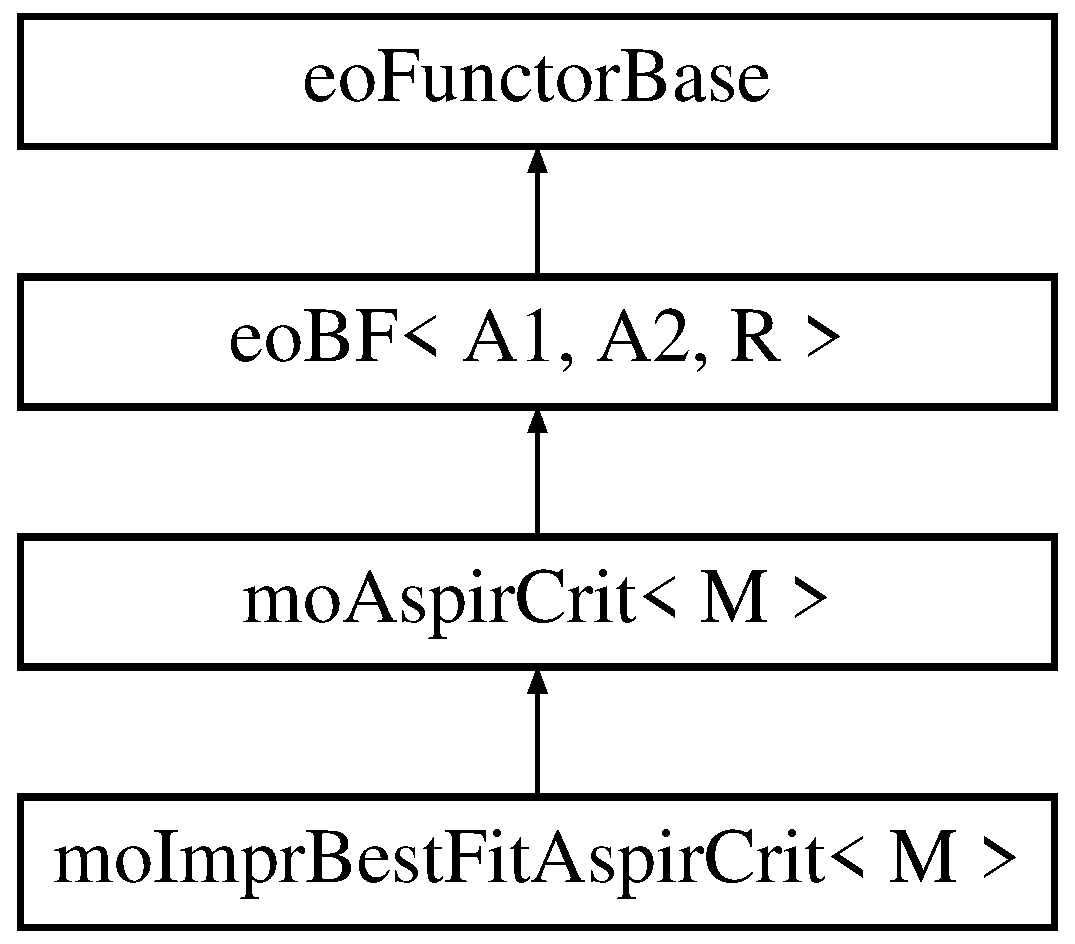
\includegraphics[height=4cm]{classmo_impr_best_fit_aspir_crit}
\end{center}
\end{figure}
\subsection*{Public Types}
\begin{CompactItemize}
\item 
typedef M::EOType::Fitness {\bf Fitness}\label{classmo_impr_best_fit_aspir_crit_0bc1a8c9af99781e662570c04750cca8}

\begin{CompactList}\small\item\em Alias for the fitness. \item\end{CompactList}\end{CompactItemize}
\subsection*{Public Member Functions}
\begin{CompactItemize}
\item 
{\bf mo\-Impr\-Best\-Fit\-Aspir\-Crit} ()\label{classmo_impr_best_fit_aspir_crit_e2c697a5cf3a7696e38bb52b6694a340}

\begin{CompactList}\small\item\em Contructor. \item\end{CompactList}\item 
void {\bf init} ()\label{classmo_impr_best_fit_aspir_crit_ffa451a14ff4ea86fb8bd9fdbc348630}

\begin{CompactList}\small\item\em Initialisation procedure. \item\end{CompactList}\item 
bool {\bf operator()} (const M \&\_\-\_\-move, const {\bf Fitness} \&\_\-\_\-fit)
\begin{CompactList}\small\item\em {\bf Function} that indicates if the fit is better that the already saved fit. \item\end{CompactList}\end{CompactItemize}
\subsection*{Private Attributes}
\begin{CompactItemize}
\item 
{\bf Fitness} {\bf best\_\-fit}\label{classmo_impr_best_fit_aspir_crit_9e52383f0af8013b4aff0942325e1bf3}

\begin{CompactList}\small\item\em Best fitness found until now. \item\end{CompactList}\item 
bool {\bf first\_\-time}\label{classmo_impr_best_fit_aspir_crit_2d5226c7dd661b33011402dbbbe78265}

\begin{CompactList}\small\item\em Indicates that a fitness has been already saved or not. \item\end{CompactList}\end{CompactItemize}


\subsection{Detailed Description}
\subsubsection*{template$<$class M$>$ class mo\-Impr\-Best\-Fit\-Aspir\-Crit$<$ M $>$}

One of the possible \doxyref{mo\-Aspir\-Crit}{p.}{classmo_aspir_crit}. 

This criterion is satisfied when a given fitness is the best ever considered. 



Definition at line 22 of file mo\-Impr\-Best\-Fit\-Aspir\-Crit.h.

\subsection{Member Function Documentation}
\index{moImprBestFitAspirCrit@{mo\-Impr\-Best\-Fit\-Aspir\-Crit}!operator()@{operator()}}
\index{operator()@{operator()}!moImprBestFitAspirCrit@{mo\-Impr\-Best\-Fit\-Aspir\-Crit}}
\subsubsection{\setlength{\rightskip}{0pt plus 5cm}template$<$class M$>$ bool {\bf mo\-Impr\-Best\-Fit\-Aspir\-Crit}$<$ M $>$::operator() (const M \& {\em \_\-\_\-move}, const {\bf Fitness} \& {\em \_\-\_\-fit})\hspace{0.3cm}{\tt  [inline]}}\label{classmo_impr_best_fit_aspir_crit_53f62fb56dcae3051a741f1fddb0204b}


{\bf Function} that indicates if the fit is better that the already saved fit. 

The first time, the function only saved the current move and fitness.

\begin{Desc}
\item[Parameters:]
\begin{description}
\item[{\em \_\-\_\-move}]a move. \item[{\em \_\-\_\-fit}]a fitnes linked to the move. \end{description}
\end{Desc}
\begin{Desc}
\item[Returns:]TRUE the first time and if \_\-\_\-fit $>$ best\_\-fit, else FALSE. \end{Desc}


Definition at line 52 of file mo\-Impr\-Best\-Fit\-Aspir\-Crit.h.

References mo\-Impr\-Best\-Fit\-Aspir\-Crit$<$ M $>$::best\_\-fit, and mo\-Impr\-Best\-Fit\-Aspir\-Crit$<$ M $>$::first\_\-time.

The documentation for this class was generated from the following file:\begin{CompactItemize}
\item 
mo\-Impr\-Best\-Fit\-Aspir\-Crit.h\end{CompactItemize}

\section{mo\-It\-Rand\-Next\-Move$<$ M $>$ Class Template Reference}
\label{classmo_it_rand_next_move}\index{moItRandNextMove@{moItRandNextMove}}
One of the possible \doxyref{mo\-Next\-Move}{p.}{classmo_next_move}.  


{\tt \#include $<$mo\-It\-Rand\-Next\-Move.h$>$}

Inheritance diagram for mo\-It\-Rand\-Next\-Move$<$ M $>$::\begin{figure}[H]
\begin{center}
\leavevmode
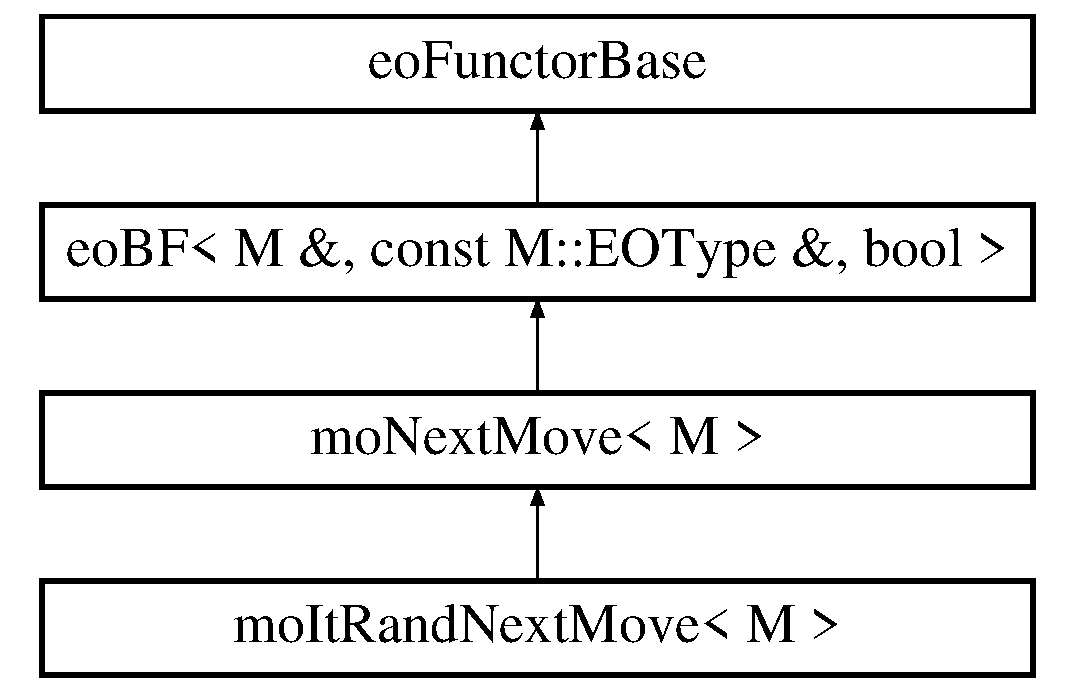
\includegraphics[height=4cm]{classmo_it_rand_next_move}
\end{center}
\end{figure}
\subsection*{Public Member Functions}
\begin{CompactItemize}
\item 
\bf{mo\-It\-Rand\-Next\-Move} (\bf{mo\-Rand\-Move}$<$ M $>$ \&\_\-\_\-rand\_\-move, unsigned int \_\-\_\-max\_\-iter)
\begin{CompactList}\small\item\em The constructor. \item\end{CompactList}\item 
bool \bf{operator()} (M \&\_\-\_\-move, const \bf{EOT} \&\_\-\_\-sol)
\begin{CompactList}\small\item\em Generation of a new move. \item\end{CompactList}\end{CompactItemize}
\subsection*{Private Types}
\begin{CompactItemize}
\item 
typedef M::EOType \bf{EOT}\label{classmo_it_rand_next_move_ee666007fc494bf4a5f0cd065e5671cf}

\begin{CompactList}\small\item\em Alias for the type. \item\end{CompactList}\end{CompactItemize}
\subsection*{Private Attributes}
\begin{CompactItemize}
\item 
\bf{mo\-Rand\-Move}$<$ M $>$ \& \bf{rand\_\-move}\label{classmo_it_rand_next_move_ef9410ec5e7dfa7f002e05967931c459}

\begin{CompactList}\small\item\em A move generator (generally randomly). \item\end{CompactList}\item 
unsigned int \bf{max\_\-iter}\label{classmo_it_rand_next_move_dc67fa86677d7a4f982de8d8b1eba033}

\begin{CompactList}\small\item\em Iteration maximum number. \item\end{CompactList}\item 
unsigned int \bf{num\_\-iter}\label{classmo_it_rand_next_move_f43494b13931d8f76b5d9d5d6469e91b}

\begin{CompactList}\small\item\em Iteration current number. \item\end{CompactList}\end{CompactItemize}


\subsection{Detailed Description}
\subsubsection*{template$<$class M$>$ class mo\-It\-Rand\-Next\-Move$<$ M $>$}

One of the possible \doxyref{mo\-Next\-Move}{p.}{classmo_next_move}. 

This class is a move (\doxyref{mo\-Move}{p.}{classmo_move}) generator with a bound for the maximum number of iterations. 



Definition at line 47 of file mo\-It\-Rand\-Next\-Move.h.

\subsection{Constructor \& Destructor Documentation}
\index{moItRandNextMove@{mo\-It\-Rand\-Next\-Move}!moItRandNextMove@{moItRandNextMove}}
\index{moItRandNextMove@{moItRandNextMove}!moItRandNextMove@{mo\-It\-Rand\-Next\-Move}}
\subsubsection{\setlength{\rightskip}{0pt plus 5cm}template$<$class M$>$ \bf{mo\-It\-Rand\-Next\-Move}$<$ M $>$::\bf{mo\-It\-Rand\-Next\-Move} (\bf{mo\-Rand\-Move}$<$ M $>$ \& {\em \_\-\_\-rand\_\-move}, unsigned int {\em \_\-\_\-max\_\-iter})\hspace{0.3cm}{\tt  [inline]}}\label{classmo_it_rand_next_move_2b61b3713d482ecf71db8d941551ff7a}


The constructor. 

\doxyref{Parameters} only for initialising the attributes.

\begin{Desc}
\item[Parameters:]
\begin{description}
\item[{\em \_\-\_\-rand\_\-move}]the random move generator. \item[{\em \_\-\_\-max\_\-iter}]the iteration maximum number. \end{description}
\end{Desc}


Definition at line 62 of file mo\-It\-Rand\-Next\-Move.h.

\subsection{Member Function Documentation}
\index{moItRandNextMove@{mo\-It\-Rand\-Next\-Move}!operator()@{operator()}}
\index{operator()@{operator()}!moItRandNextMove@{mo\-It\-Rand\-Next\-Move}}
\subsubsection{\setlength{\rightskip}{0pt plus 5cm}template$<$class M$>$ bool \bf{mo\-It\-Rand\-Next\-Move}$<$ M $>$::operator() (M \& {\em \_\-\_\-move}, const \bf{EOT} \& {\em \_\-\_\-sol})\hspace{0.3cm}{\tt  [inline]}}\label{classmo_it_rand_next_move_92a2fbbc02a20853b9a309e99018a102}


Generation of a new move. 

If the maximum number is not already reached, the current move is forgotten and remplaced by another one.

\begin{Desc}
\item[Parameters:]
\begin{description}
\item[{\em \_\-\_\-move}]the current move. \item[{\em \_\-\_\-sol}]the current solution. \end{description}
\end{Desc}
\begin{Desc}
\item[Returns:]FALSE if the maximum number of iteration is reached, else TRUE. \end{Desc}


Definition at line 77 of file mo\-It\-Rand\-Next\-Move.h.

References mo\-It\-Rand\-Next\-Move$<$ M $>$::max\_\-iter, mo\-It\-Rand\-Next\-Move$<$ M $>$::num\_\-iter, and mo\-It\-Rand\-Next\-Move$<$ M $>$::rand\_\-move.

The documentation for this class was generated from the following file:\begin{CompactItemize}
\item 
mo\-It\-Rand\-Next\-Move.h\end{CompactItemize}

\section{mo\-Linear\-Cooling\-Schedule Class Reference}
\label{classmo_linear_cooling_schedule}\index{moLinearCoolingSchedule@{moLinearCoolingSchedule}}
One of the possible {\bf mo\-Cooling\-Schedule}{\rm (p.\,\pageref{classmo_cooling_schedule})}.  


{\tt \#include $<$mo\-Linear\-Cooling\-Schedule.h$>$}

Inheritance diagram for mo\-Linear\-Cooling\-Schedule::\begin{figure}[H]
\begin{center}
\leavevmode
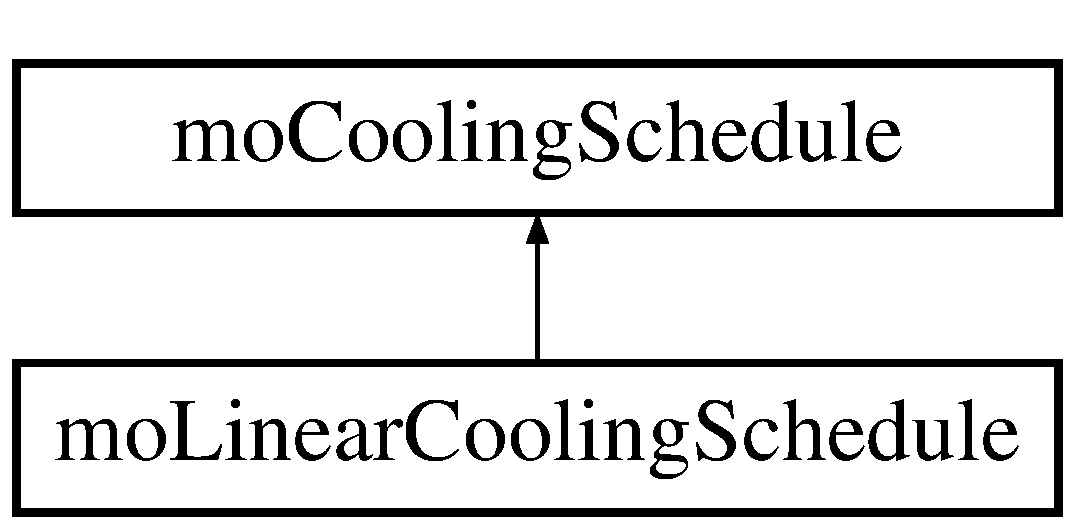
\includegraphics[height=4cm]{classmo_linear_cooling_schedule}
\end{center}
\end{figure}
\subsection*{Public Member Functions}
\begin{CompactItemize}
\item 
{\bf mo\-Linear\-Cooling\-Schedule} (double \_\-threshold, double \_\-quantity)
\begin{CompactList}\small\item\em Simple constructor. \item\end{CompactList}\item 
bool {\bf operator()} (double \&\_\-current\_\-temperature)
\begin{CompactList}\small\item\em Function which proceeds to the cooling. \item\end{CompactList}\end{CompactItemize}
\subsection*{Private Attributes}
\begin{CompactItemize}
\item 
double {\bf threshold}\label{classmo_linear_cooling_schedule_r0}

\begin{CompactList}\small\item\em The temperature threhold. \item\end{CompactList}\item 
double {\bf quantity}\label{classmo_linear_cooling_schedule_r1}

\begin{CompactList}\small\item\em The quantity that allows the temperature to decrease. \item\end{CompactList}\end{CompactItemize}


\subsection{Detailed Description}
One of the possible {\bf mo\-Cooling\-Schedule}{\rm (p.\,\pageref{classmo_cooling_schedule})}. 

An another very simple cooling schedule, the temperature decrease according to a quantity while the temperature is greater than a threshold. 



Definition at line 46 of file mo\-Linear\-Cooling\-Schedule.h.

\subsection{Constructor \& Destructor Documentation}
\index{moLinearCoolingSchedule@{mo\-Linear\-Cooling\-Schedule}!moLinearCoolingSchedule@{moLinearCoolingSchedule}}
\index{moLinearCoolingSchedule@{moLinearCoolingSchedule}!moLinearCoolingSchedule@{mo\-Linear\-Cooling\-Schedule}}
\subsubsection{\setlength{\rightskip}{0pt plus 5cm}mo\-Linear\-Cooling\-Schedule::mo\-Linear\-Cooling\-Schedule (double {\em \_\-threshold}, double {\em \_\-quantity})\hspace{0.3cm}{\tt  [inline]}}\label{classmo_linear_cooling_schedule_a0}


Simple constructor. 

\begin{Desc}
\item[Parameters:]
\begin{description}
\item[{\em \_\-threshold}]the threshold. \item[{\em \_\-quantity}]the quantity used to descrease the temperature. \end{description}
\end{Desc}


Definition at line 55 of file mo\-Linear\-Cooling\-Schedule.h.

References quantity, and threshold.

\subsection{Member Function Documentation}
\index{moLinearCoolingSchedule@{mo\-Linear\-Cooling\-Schedule}!operator()@{operator()}}
\index{operator()@{operator()}!moLinearCoolingSchedule@{mo\-Linear\-Cooling\-Schedule}}
\subsubsection{\setlength{\rightskip}{0pt plus 5cm}bool mo\-Linear\-Cooling\-Schedule::operator() (double \& {\em \_\-current\_\-temperature})\hspace{0.3cm}{\tt  [inline, virtual]}}\label{classmo_linear_cooling_schedule_a1}


Function which proceeds to the cooling. 

It decreases the temperature and indicates if it is greater than the threshold.

\begin{Desc}
\item[Parameters:]
\begin{description}
\item[{\em \_\-current\_\-temperature}]The current temperature. \end{description}
\end{Desc}
\begin{Desc}
\item[Returns:]true if the new temperature (current temperature - quantity) is greater than the threshold, false otherwise. \end{Desc}


Implements {\bf eo\-UF$<$ double \&, bool $>$}.

Definition at line 65 of file mo\-Linear\-Cooling\-Schedule.h.

The documentation for this class was generated from the following file:\begin{CompactItemize}
\item 
mo\-Linear\-Cooling\-Schedule.h\end{CompactItemize}

\section{mo\-LSCheck\-Point$<$ M $>$ Class Template Reference}
\label{classmo_l_s_check_point}\index{moLSCheckPoint@{moLSCheckPoint}}
Class which allows a checkpointing system.  


{\tt \#include $<$mo\-LSCheck\-Point.h$>$}

\subsection*{Public Member Functions}
\begin{CompactItemize}
\item 
void {\bf operator()} (const M \&\_\-\_\-move, const typename M::EOType \&\_\-\_\-sol)
\begin{CompactList}\small\item\em Function which launches the checkpointing. \item\end{CompactList}\item 
void {\bf add} (eo\-BF$<$ const M \&, const typename M::EOType \&, void $>$ \&\_\-\_\-f)
\begin{CompactList}\small\item\em Procedure which add a new function to the function vector. \item\end{CompactList}\end{CompactItemize}
\subsection*{Private Attributes}
\begin{CompactItemize}
\item 
std::vector$<$ eo\-BF$<$ const M \&, const typename M::EOType \&, void $>$ $\ast$ $>$ {\bf func}\label{classmo_l_s_check_point_ff2a31ee5689a804bd9a572c51a36ca4}

\begin{CompactList}\small\item\em vector of function \item\end{CompactList}\end{CompactItemize}


\subsection{Detailed Description}
\subsubsection*{template$<$class M$>$ class mo\-LSCheck\-Point$<$ M $>$}

Class which allows a checkpointing system. 

Thanks to this class, at each iteration, additionnal function can be used (and not only one). 



Definition at line 21 of file mo\-LSCheck\-Point.h.

\subsection{Member Function Documentation}
\index{moLSCheckPoint@{mo\-LSCheck\-Point}!operator()@{operator()}}
\index{operator()@{operator()}!moLSCheckPoint@{mo\-LSCheck\-Point}}
\subsubsection{\setlength{\rightskip}{0pt plus 5cm}template$<$class M$>$ void {\bf mo\-LSCheck\-Point}$<$ M $>$::operator() (const M \& {\em \_\-\_\-move}, const typename M::EOType \& {\em \_\-\_\-sol})\hspace{0.3cm}{\tt  [inline]}}\label{classmo_l_s_check_point_2f9c1250279e3f49ec77a66c10029f1e}


Function which launches the checkpointing. 

Each saved function is used on the current move and the current solution.

\begin{Desc}
\item[Parameters:]
\begin{description}
\item[{\em \_\-\_\-move}]a move. \item[{\em \_\-\_\-sol}]a solution. \end{description}
\end{Desc}


Definition at line 34 of file mo\-LSCheck\-Point.h.

References mo\-LSCheck\-Point$<$ M $>$::func.\index{moLSCheckPoint@{mo\-LSCheck\-Point}!add@{add}}
\index{add@{add}!moLSCheckPoint@{mo\-LSCheck\-Point}}
\subsubsection{\setlength{\rightskip}{0pt plus 5cm}template$<$class M$>$ void {\bf mo\-LSCheck\-Point}$<$ M $>$::add (eo\-BF$<$ const M \&, const typename M::EOType \&, void $>$ \& {\em \_\-\_\-f})\hspace{0.3cm}{\tt  [inline]}}\label{classmo_l_s_check_point_66be5fe2944bcdd752f1e58105e969a6}


Procedure which add a new function to the function vector. 

The new function is added at the end of the vector. \begin{Desc}
\item[Parameters:]
\begin{description}
\item[{\em \_\-\_\-f}]a new function to add. \end{description}
\end{Desc}


Definition at line 49 of file mo\-LSCheck\-Point.h.

References mo\-LSCheck\-Point$<$ M $>$::func.

The documentation for this class was generated from the following file:\begin{CompactItemize}
\item 
mo\-LSCheck\-Point.h\end{CompactItemize}

\section{mo\-Move$<$ EOT $>$ Class Template Reference}
\label{classmo_move}\index{moMove@{moMove}}
Definition of a move.  


{\tt \#include $<$mo\-Move.h$>$}

\subsection*{Public Types}
\begin{CompactItemize}
\item 
typedef EOT \bf{EOType}\label{classmo_move_7fb853a91ba1319530529e515380bbba}

\begin{CompactList}\small\item\em Alias for the type. \item\end{CompactList}\end{CompactItemize}


\subsection{Detailed Description}
\subsubsection*{template$<$class EOT$>$ class mo\-Move$<$ EOT $>$}

Definition of a move. 

A move transforms a solution to another close solution. It describes how a solution can be modified to another one. 



Definition at line 23 of file mo\-Move.h.

The documentation for this class was generated from the following file:\begin{CompactItemize}
\item 
mo\-Move.h\end{CompactItemize}

\section{mo\-Move\-Expl$<$ M $>$ Class Template Reference}
\label{classmo_move_expl}\index{moMoveExpl@{moMoveExpl}}
Description of a move (\doxyref{mo\-Move}{p.}{classmo_move}) explorer.  


{\tt \#include $<$mo\-Move\-Expl.h$>$}

Inheritance diagram for mo\-Move\-Expl$<$ M $>$::\begin{figure}[H]
\begin{center}
\leavevmode
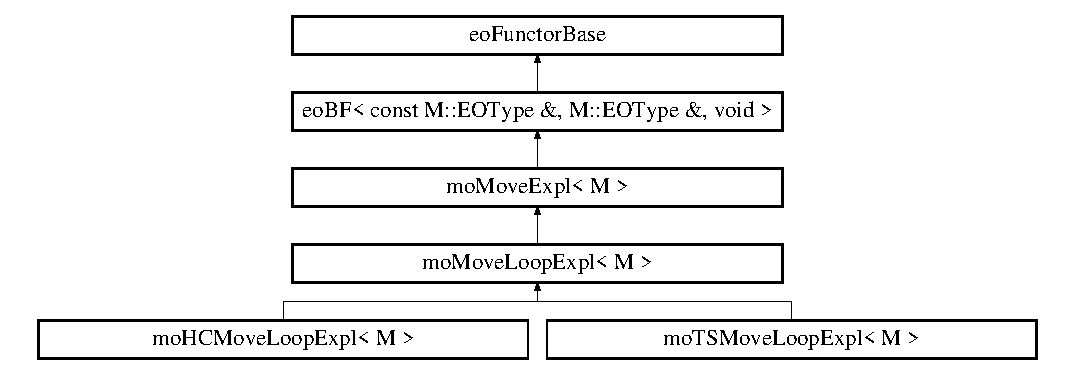
\includegraphics[height=4.59016cm]{classmo_move_expl}
\end{center}
\end{figure}


\subsection{Detailed Description}
\subsubsection*{template$<$class M$>$ class mo\-Move\-Expl$<$ M $>$}

Description of a move (\doxyref{mo\-Move}{p.}{classmo_move}) explorer. 

Only a description...See \doxyref{mo\-Move\-Loop\-Expl}{p.}{classmo_move_loop_expl}. 



Definition at line 46 of file mo\-Move\-Expl.h.

The documentation for this class was generated from the following file:\begin{CompactItemize}
\item 
mo\-Move\-Expl.h\end{CompactItemize}

\section{moMoveIncrEval$<$ M $>$ Class Template Reference}
\label{classmo_move_incr_eval}\index{moMoveIncrEval@{moMoveIncrEval}}
(generally) Efficient evaluation function based a move and a solution.  


{\tt \#include $<$moMoveIncrEval.h$>$}

Inheritance diagram for moMoveIncrEval$<$ M $>$::\begin{figure}[H]
\begin{center}
\leavevmode
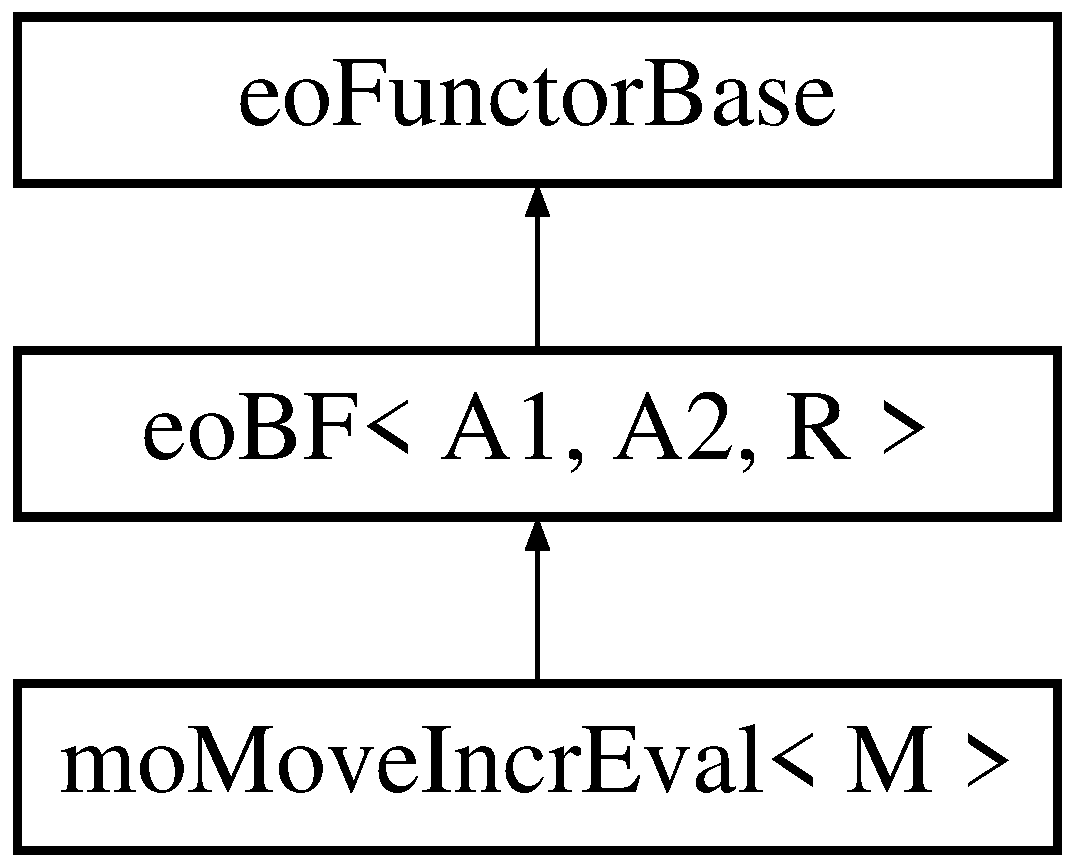
\includegraphics[height=3cm]{classmo_move_incr_eval}
\end{center}
\end{figure}


\subsection{Detailed Description}
\subsubsection*{template$<$class M$>$ class moMoveIncrEval$<$ M $>$}

(generally) Efficient evaluation function based a move and a solution. 

From a move and a solution, it computes a new fitness that could be associated to the solution if this one is updated. 



Definition at line 24 of file moMoveIncrEval.h.

The documentation for this class was generated from the following file:\begin{CompactItemize}
\item 
moMoveIncrEval.h\end{CompactItemize}

\section{moMoveInit$<$ M $>$ Class Template Reference}
\label{classmo_move_init}\index{moMoveInit@{moMoveInit}}
Move (\doxyref{moMove}{p.}{classmo_move}) initializer.  


{\tt \#include $<$moMoveInit.h$>$}

Inheritance diagram for moMoveInit$<$ M $>$::\begin{figure}[H]
\begin{center}
\leavevmode
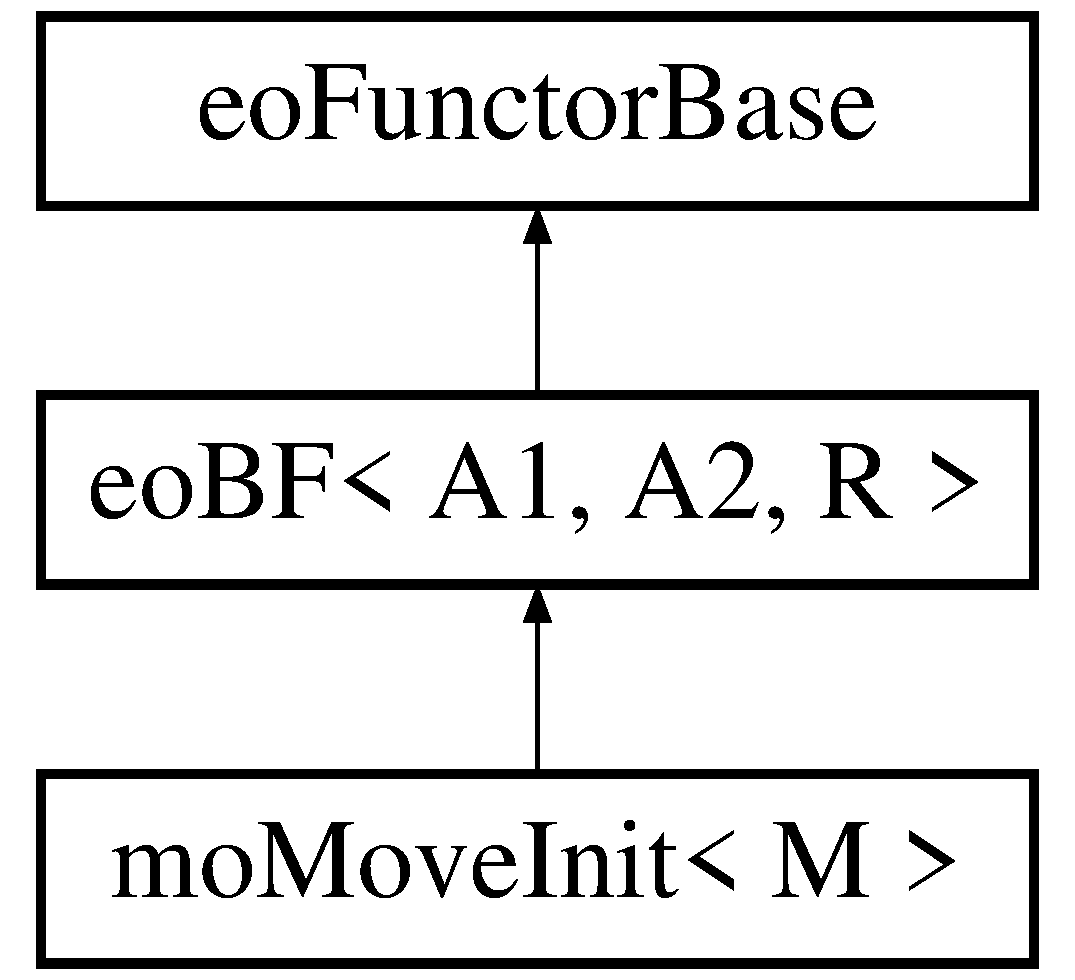
\includegraphics[height=3cm]{classmo_move_init}
\end{center}
\end{figure}


\subsection{Detailed Description}
\subsubsection*{template$<$class M$>$ class moMoveInit$<$ M $>$}

Move (\doxyref{moMove}{p.}{classmo_move}) initializer. 

Class which allows to initiase a move. Only a description... An object that herits from this class needs to be designed to be used. 



Definition at line 45 of file moMoveInit.h.

The documentation for this class was generated from the following file:\begin{CompactItemize}
\item 
moMoveInit.h\end{CompactItemize}

\section{mo\-Move\-Loop\-Expl$<$ M $>$ Class Template Reference}
\label{classmo_move_loop_expl}\index{moMoveLoopExpl@{moMoveLoopExpl}}
Class which describes an iterative explorer.  


{\tt \#include $<$mo\-Move\-Loop\-Expl.h$>$}

Inheritance diagram for mo\-Move\-Loop\-Expl$<$ M $>$::\begin{figure}[H]
\begin{center}
\leavevmode
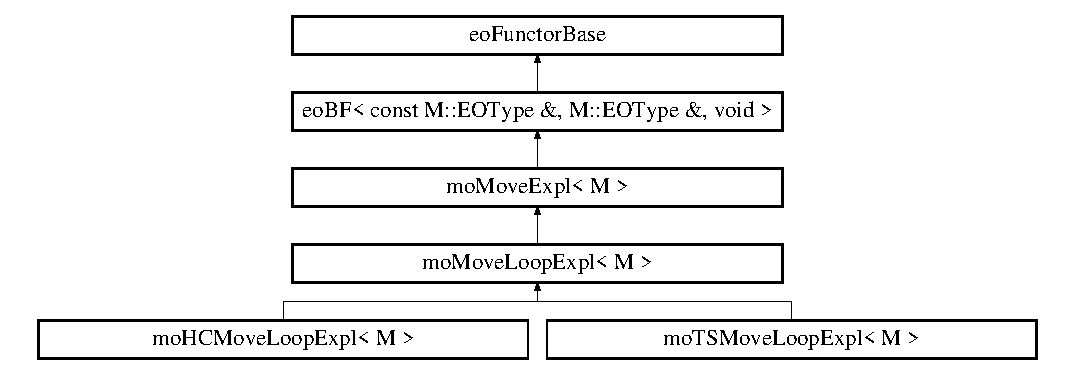
\includegraphics[height=3cm]{classmo_move_loop_expl}
\end{center}
\end{figure}


\subsection{Detailed Description}
\subsubsection*{template$<$class M$>$ class mo\-Move\-Loop\-Expl$<$ M $>$}

Class which describes an iterative explorer. 

Only a description... \doxyref{mo\-HCMove\-Loop\-Expl}{p.}{classmo_h_c_move_loop_expl} and \doxyref{mo\-TSMove\-Loop\-Expl}{p.}{classmo_t_s_move_loop_expl} are exemples of class that are a \doxyref{mo\-Move\-Loop\-Expl}{p.}{classmo_move_loop_expl}. 



Definition at line 47 of file mo\-Move\-Loop\-Expl.h.

The documentation for this class was generated from the following file:\begin{CompactItemize}
\item 
mo\-Move\-Loop\-Expl.h\end{CompactItemize}

\section{mo\-Move\-Select$<$ M $>$ Class Template Reference}
\label{classmo_move_select}\index{moMoveSelect@{moMoveSelect}}
Class that describes a move selector (\doxyref{mo\-Move}{p.}{classmo_move}).  


{\tt \#include $<$mo\-Move\-Select.h$>$}

Inheritance diagram for mo\-Move\-Select$<$ M $>$::\begin{figure}[H]
\begin{center}
\leavevmode
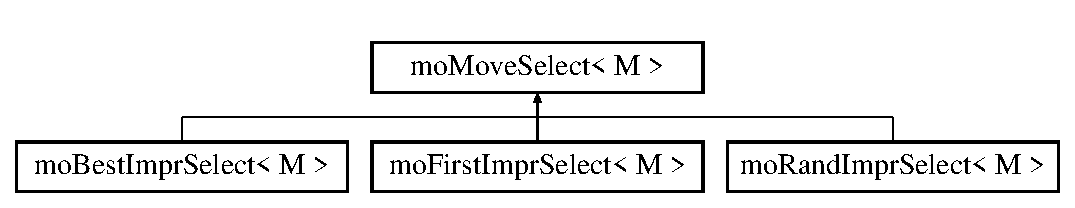
\includegraphics[height=2cm]{classmo_move_select}
\end{center}
\end{figure}
\subsection*{Public Types}
\begin{CompactItemize}
\item 
typedef M::EOType::Fitness \bf{Fitness}\label{classmo_move_select_8148ccc0e6fbd209c3fe6829559895c8}

\begin{CompactList}\small\item\em Alias for the fitness. \item\end{CompactList}\end{CompactItemize}
\subsection*{Public Member Functions}
\begin{CompactItemize}
\item 
virtual void \bf{init} (const \bf{Fitness} \&\_\-\_\-fit)=0
\begin{CompactList}\small\item\em Procedure which initialises all that the move selector needs including the initial fitness. \item\end{CompactList}\item 
virtual bool \bf{update} (const M \&\_\-\_\-move, const \bf{Fitness} \&\_\-\_\-fit)=0
\begin{CompactList}\small\item\em Function which updates the best solutions. \item\end{CompactList}\end{CompactItemize}


\subsection{Detailed Description}
\subsubsection*{template$<$class M$>$ class mo\-Move\-Select$<$ M $>$}

Class that describes a move selector (\doxyref{mo\-Move}{p.}{classmo_move}). 

It iteratively considers some moves (\doxyref{mo\-Move}{p.}{classmo_move}) and their associated fitnesses. The best move is so regularly updated. At any time, it could be accessed. 



Definition at line 32 of file mo\-Move\-Select.h.

\subsection{Member Function Documentation}
\index{moMoveSelect@{mo\-Move\-Select}!init@{init}}
\index{init@{init}!moMoveSelect@{mo\-Move\-Select}}
\subsubsection{\setlength{\rightskip}{0pt plus 5cm}template$<$class M$>$ virtual void \bf{mo\-Move\-Select}$<$ M $>$::init (const \bf{Fitness} \& {\em \_\-\_\-fit})\hspace{0.3cm}{\tt  [pure virtual]}}\label{classmo_move_select_bca4c43f13d26eca7163aeb272a4a52e}


Procedure which initialises all that the move selector needs including the initial fitness. 

In order to know the fitness of the solution, for which the neighborhood will be soon explored

\begin{Desc}
\item[Parameters:]
\begin{description}
\item[{\em \_\-\_\-fit}]the current fitness. \end{description}
\end{Desc}


Implemented in \bf{mo\-Best\-Impr\-Select$<$ M $>$} \doxyref{p.}{classmo_best_impr_select_2d2abf9aa17dc77cbb4f41810ab7b956}, \bf{mo\-First\-Impr\-Select$<$ M $>$} \doxyref{p.}{classmo_first_impr_select_4c5ce18ede46247a439c68f6954a4055}, and \bf{mo\-Rand\-Impr\-Select$<$ M $>$} \doxyref{p.}{classmo_rand_impr_select_a19726a1509cff874801615d63a3b5d9}.\index{moMoveSelect@{mo\-Move\-Select}!update@{update}}
\index{update@{update}!moMoveSelect@{mo\-Move\-Select}}
\subsubsection{\setlength{\rightskip}{0pt plus 5cm}template$<$class M$>$ virtual bool \bf{mo\-Move\-Select}$<$ M $>$::update (const M \& {\em \_\-\_\-move}, const \bf{Fitness} \& {\em \_\-\_\-fit})\hspace{0.3cm}{\tt  [pure virtual]}}\label{classmo_move_select_7c157b6e64fd417acf6e900059204eb1}


Function which updates the best solutions. 

\begin{Desc}
\item[Parameters:]
\begin{description}
\item[{\em \_\-\_\-move}]a new move. \item[{\em \_\-\_\-fit}]a fitness linked to the new move. \end{description}
\end{Desc}
\begin{Desc}
\item[Returns:]a boolean that expresses the need to resume the exploration. \end{Desc}


Implemented in \bf{mo\-Best\-Impr\-Select$<$ M $>$} \doxyref{p.}{classmo_best_impr_select_d10e3e6f8a0277731e95ef506d064d6d}, and \bf{mo\-Rand\-Impr\-Select$<$ M $>$} \doxyref{p.}{classmo_rand_impr_select_60ae5548560caee7e28d5ed2446186c9}.

The documentation for this class was generated from the following file:\begin{CompactItemize}
\item 
mo\-Move\-Select.h\end{CompactItemize}

\section{moNextMove$<$ M $>$ Class Template Reference}
\label{classmo_next_move}\index{moNextMove@{moNextMove}}
Class which allows to generate a new move (\doxyref{moMove}{p.}{classmo_move}).  


{\tt \#include $<$moNextMove.h$>$}

Inheritance diagram for moNextMove$<$ M $>$::\begin{figure}[H]
\begin{center}
\leavevmode
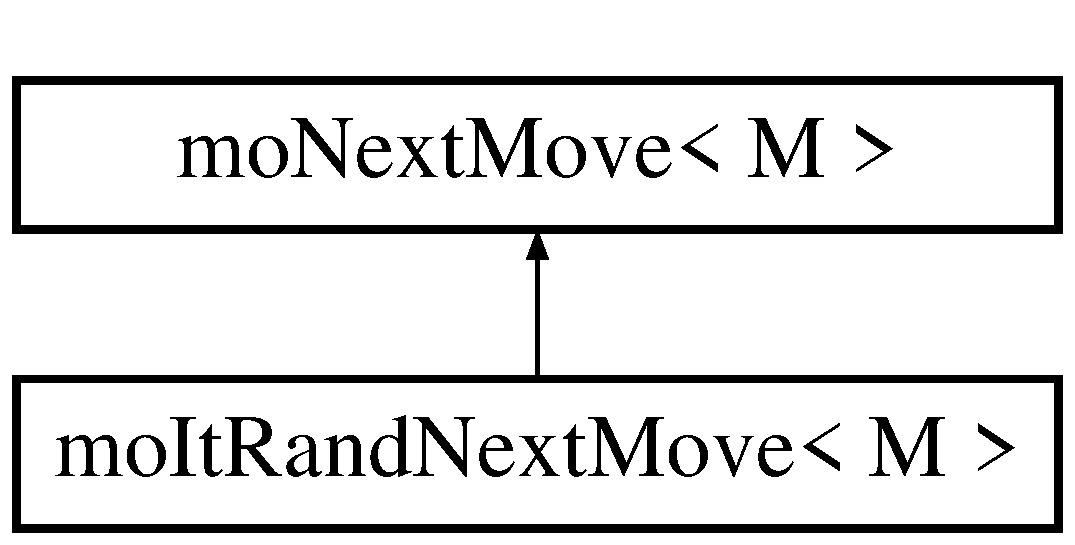
\includegraphics[height=2cm]{classmo_next_move}
\end{center}
\end{figure}


\subsection{Detailed Description}
\subsubsection*{template$<$class M$>$ class moNextMove$<$ M $>$}

Class which allows to generate a new move (\doxyref{moMove}{p.}{classmo_move}). 

Useful for the explorer (for \doxyref{moTS}{p.}{classmo_t_s} or \doxyref{moHC}{p.}{classmo_h_c}). Does nothing... An object that herits from this class needs to be designed for being used. 



Definition at line 22 of file moNextMove.h.

The documentation for this class was generated from the following file:\begin{CompactItemize}
\item 
moNextMove.h\end{CompactItemize}

\section{mo\-No\-Aspir\-Crit$<$ M $>$ Class Template Reference}
\label{classmo_no_aspir_crit}\index{moNoAspirCrit@{moNoAspirCrit}}
One of the possible aspiration criterion (\doxyref{mo\-Aspir\-Crit}{p.}{classmo_aspir_crit}).  


{\tt \#include $<$mo\-No\-Aspir\-Crit.h$>$}

Inheritance diagram for mo\-No\-Aspir\-Crit$<$ M $>$::\begin{figure}[H]
\begin{center}
\leavevmode
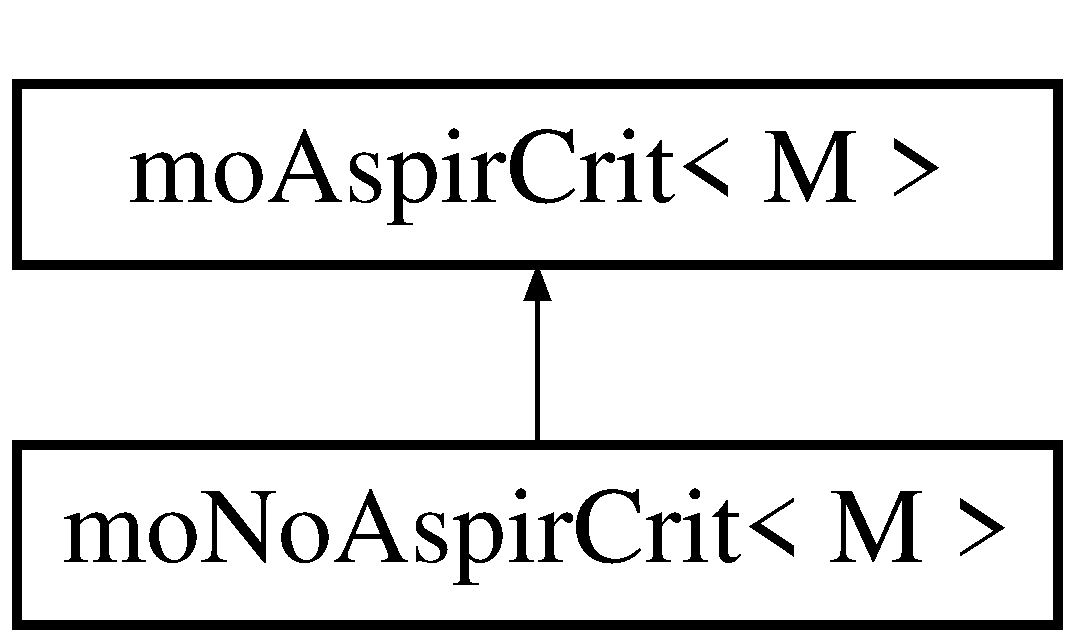
\includegraphics[height=4cm]{classmo_no_aspir_crit}
\end{center}
\end{figure}
\subsection*{Private Member Functions}
\begin{CompactItemize}
\item 
bool \bf{operator()} (const M \&\_\-\_\-move, const typename M::EOType::Fitness \&\_\-\_\-sol)
\begin{CompactList}\small\item\em \doxyref{Function} which describes the aspiration criterion behaviour. \item\end{CompactList}\item 
void \bf{init} ()
\begin{CompactList}\small\item\em Procedure which initialises all that needs a \doxyref{mo\-No\-Aspir\-Crit}{p.}{classmo_no_aspir_crit}. \item\end{CompactList}\end{CompactItemize}


\subsection{Detailed Description}
\subsubsection*{template$<$class M$>$ class mo\-No\-Aspir\-Crit$<$ M $>$}

One of the possible aspiration criterion (\doxyref{mo\-Aspir\-Crit}{p.}{classmo_aspir_crit}). 

The simplest : never satisfied. 



Definition at line 21 of file mo\-No\-Aspir\-Crit.h.

\subsection{Member Function Documentation}
\index{moNoAspirCrit@{mo\-No\-Aspir\-Crit}!operator()@{operator()}}
\index{operator()@{operator()}!moNoAspirCrit@{mo\-No\-Aspir\-Crit}}
\subsubsection{\setlength{\rightskip}{0pt plus 5cm}template$<$class M$>$ bool \bf{mo\-No\-Aspir\-Crit}$<$ M $>$::operator() (const M \& {\em \_\-\_\-move}, const typename M::EOType::Fitness \& {\em \_\-\_\-sol})\hspace{0.3cm}{\tt  [inline, private]}}\label{classmo_no_aspir_crit_8a7180a8d5c25bfb6727d0b59551b0f8}


\doxyref{Function} which describes the aspiration criterion behaviour. 

Does nothing.

\begin{Desc}
\item[Parameters:]
\begin{description}
\item[{\em \_\-\_\-move}]a move. \item[{\em \_\-\_\-sol}]a fitness. \end{description}
\end{Desc}
\begin{Desc}
\item[Returns:]FALSE. \end{Desc}


Definition at line 32 of file mo\-No\-Aspir\-Crit.h.\index{moNoAspirCrit@{mo\-No\-Aspir\-Crit}!init@{init}}
\index{init@{init}!moNoAspirCrit@{mo\-No\-Aspir\-Crit}}
\subsubsection{\setlength{\rightskip}{0pt plus 5cm}template$<$class M$>$ void \bf{mo\-No\-Aspir\-Crit}$<$ M $>$::init ()\hspace{0.3cm}{\tt  [inline, private, virtual]}}\label{classmo_no_aspir_crit_f3a286fc4c2d36bd390ba9a3074f3037}


Procedure which initialises all that needs a \doxyref{mo\-No\-Aspir\-Crit}{p.}{classmo_no_aspir_crit}. 

Nothing... 

Implements \bf{mo\-Aspir\-Crit$<$ M $>$} \doxyref{p.}{classmo_aspir_crit_a8ce84510a5ec7c9078381e542c6d140}.

Definition at line 43 of file mo\-No\-Aspir\-Crit.h.

The documentation for this class was generated from the following file:\begin{CompactItemize}
\item 
mo\-No\-Aspir\-Crit.h\end{CompactItemize}

\section{moRandImprSelect$<$ M $>$ Class Template Reference}
\label{classmo_rand_impr_select}\index{moRandImprSelect@{moRandImprSelect}}
One of the possible \doxyref{moMove}{p.}{classmo_move} selector (\doxyref{moMoveSelect}{p.}{classmo_move_select}).  


{\tt \#include $<$moRandImprSelect.h$>$}

Inheritance diagram for moRandImprSelect$<$ M $>$::\begin{figure}[H]
\begin{center}
\leavevmode
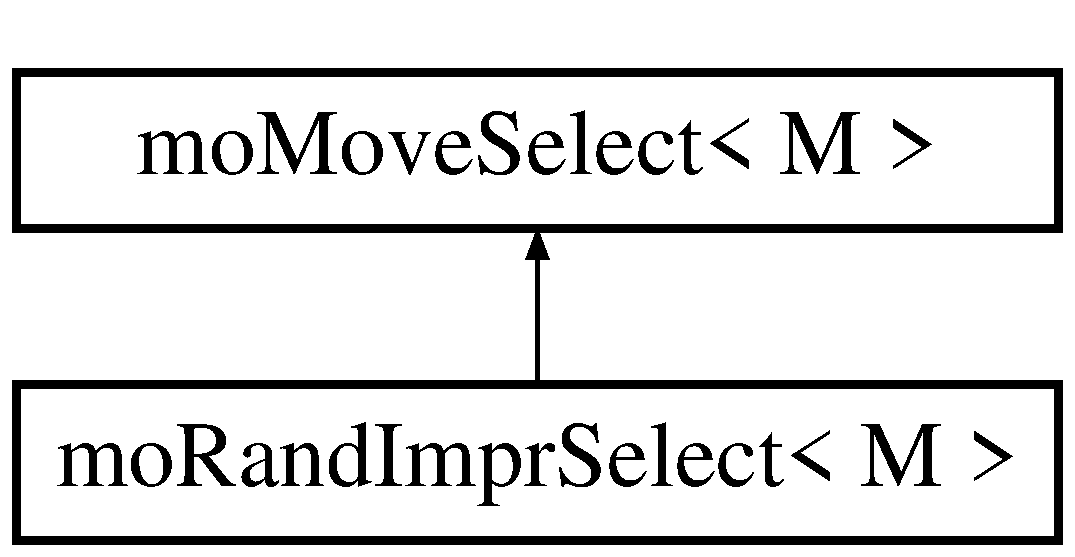
\includegraphics[height=4cm]{classmo_rand_impr_select}
\end{center}
\end{figure}
\subsection*{Public Types}
\begin{CompactItemize}
\item 
typedef M::EOType::Fitness {\bf Fitness}\label{classmo_rand_impr_select_3bff2fdb963297430543c82ffb567a5c}

\begin{CompactList}\small\item\em Alias for the fitness. \item\end{CompactList}\end{CompactItemize}
\subsection*{Public Member Functions}
\begin{CompactItemize}
\item 
void {\bf init} (const {\bf Fitness} \&\_\-\_\-fit)
\begin{CompactList}\small\item\em Procedure which all that needs a \doxyref{moRandImprSelect}{p.}{classmo_rand_impr_select}. \item\end{CompactList}\item 
bool {\bf update} (const M \&\_\-\_\-move, const {\bf Fitness} \&\_\-\_\-fit)
\begin{CompactList}\small\item\em {\bf Function} that updates the fitness and move vectors. \item\end{CompactList}\item 
void {\bf operator()} (M \&\_\-\_\-move, {\bf Fitness} \&\_\-\_\-fit)  throw (EmptySelection)
\begin{CompactList}\small\item\em The move selection. \item\end{CompactList}\end{CompactItemize}
\subsection*{Private Attributes}
\begin{CompactItemize}
\item 
{\bf Fitness} {\bf init\_\-fit}\label{classmo_rand_impr_select_d153c277a0a2ea95ac484210d445b40e}

\begin{CompactList}\small\item\em Fitness of the current solution. \item\end{CompactList}\item 
std::vector$<$ {\bf Fitness} $>$ {\bf vect\_\-better\_\-fit}\label{classmo_rand_impr_select_05c7c3b858e8a25632f2f5c86b0c97a3}

\begin{CompactList}\small\item\em Candidate fitnesse vector. \item\end{CompactList}\item 
std::vector$<$ M $>$ {\bf vect\_\-better\_\-moves}\label{classmo_rand_impr_select_2ace12bd179144fa71d56324694201f5}

\begin{CompactList}\small\item\em Candidate move vector. \item\end{CompactList}\end{CompactItemize}


\subsection{Detailed Description}
\subsubsection*{template$<$class M$>$ class moRandImprSelect$<$ M $>$}

One of the possible \doxyref{moMove}{p.}{classmo_move} selector (\doxyref{moMoveSelect}{p.}{classmo_move_select}). 

All the neighbors are considered. One of them that enables an improvment of the objective function is choosen. 



Definition at line 25 of file moRandImprSelect.h.

\subsection{Member Function Documentation}
\index{moRandImprSelect@{moRandImprSelect}!init@{init}}
\index{init@{init}!moRandImprSelect@{moRandImprSelect}}
\subsubsection{\setlength{\rightskip}{0pt plus 5cm}template$<$class M$>$ void {\bf moRandImprSelect}$<$ M $>$::init (const {\bf Fitness} \& {\em \_\-\_\-fit})\hspace{0.3cm}{\tt  [inline, virtual]}}\label{classmo_rand_impr_select_a19726a1509cff874801615d63a3b5d9}


Procedure which all that needs a \doxyref{moRandImprSelect}{p.}{classmo_rand_impr_select}. 

Give a value to the initialise fitness. Clean the move and fitness vectors.

\begin{Desc}
\item[Parameters:]
\begin{description}
\item[{\em \_\-\_\-fit}]the current best fitness \end{description}
\end{Desc}


Implements {\bf moMoveSelect$<$ M $>$} \doxyref{}{p.}{classmo_move_select_bca4c43f13d26eca7163aeb272a4a52e}.

Definition at line 40 of file moRandImprSelect.h.

References moRandImprSelect$<$ M $>$::init\_\-fit, moRandImprSelect$<$ M $>$::vect\_\-better\_\-fit, and moRandImprSelect$<$ M $>$::vect\_\-better\_\-moves.\index{moRandImprSelect@{moRandImprSelect}!update@{update}}
\index{update@{update}!moRandImprSelect@{moRandImprSelect}}
\subsubsection{\setlength{\rightskip}{0pt plus 5cm}template$<$class M$>$ bool {\bf moRandImprSelect}$<$ M $>$::update (const M \& {\em \_\-\_\-move}, const {\bf Fitness} \& {\em \_\-\_\-fit})\hspace{0.3cm}{\tt  [inline, virtual]}}\label{classmo_rand_impr_select_60ae5548560caee7e28d5ed2446186c9}


{\bf Function} that updates the fitness and move vectors. 

if a move give a better fitness than the initial fitness, it is saved and the fitness too.

\begin{Desc}
\item[Parameters:]
\begin{description}
\item[{\em \_\-\_\-move}]a new move. \item[{\em \_\-\_\-fit}]a new fitness associated to the new move. \end{description}
\end{Desc}
\begin{Desc}
\item[Returns:]TRUE. \end{Desc}


Implements {\bf moMoveSelect$<$ M $>$} \doxyref{}{p.}{classmo_move_select_7c157b6e64fd417acf6e900059204eb1}.

Definition at line 56 of file moRandImprSelect.h.

References moRandImprSelect$<$ M $>$::init\_\-fit, moRandImprSelect$<$ M $>$::vect\_\-better\_\-fit, and moRandImprSelect$<$ M $>$::vect\_\-better\_\-moves.\index{moRandImprSelect@{moRandImprSelect}!operator()@{operator()}}
\index{operator()@{operator()}!moRandImprSelect@{moRandImprSelect}}
\subsubsection{\setlength{\rightskip}{0pt plus 5cm}template$<$class M$>$ void {\bf moRandImprSelect}$<$ M $>$::operator() (M \& {\em \_\-\_\-move}, {\bf Fitness} \& {\em \_\-\_\-fit})  throw ({\bf EmptySelection})\hspace{0.3cm}{\tt  [inline, virtual]}}\label{classmo_rand_impr_select_5ee57f77a450c0a9ce50bfccf3ad2a55}


The move selection. 

One the saved move is randomly chosen.

\begin{Desc}
\item[Parameters:]
\begin{description}
\item[{\em \_\-\_\-move}]the reference of the move that can be initialised by the function. \item[{\em \_\-\_\-fit}]the reference of the fitness that can be initialised by the function. \end{description}
\end{Desc}
\begin{Desc}
\item[Exceptions:]
\begin{description}
\item[{\em \doxyref{EmptySelection}{p.}{class_empty_selection}}]If no move which improves the current fitness are found. \end{description}
\end{Desc}


Implements {\bf eoBF$<$ M \&, M::EOType::Fitness \&, void $>$}.

Definition at line 77 of file moRandImprSelect.h.

References eoRng::random(), moRandImprSelect$<$ M $>$::vect\_\-better\_\-fit, and moRandImprSelect$<$ M $>$::vect\_\-better\_\-moves.

The documentation for this class was generated from the following file:\begin{CompactItemize}
\item 
moRandImprSelect.h\end{CompactItemize}

\section{moRandMove$<$ M $>$ Class Template Reference}
\label{classmo_rand_move}\index{moRandMove@{moRandMove}}
Random move generator.  


{\tt \#include $<$moRandMove.h$>$}

Inheritance diagram for moRandMove$<$ M $>$::\begin{figure}[H]
\begin{center}
\leavevmode
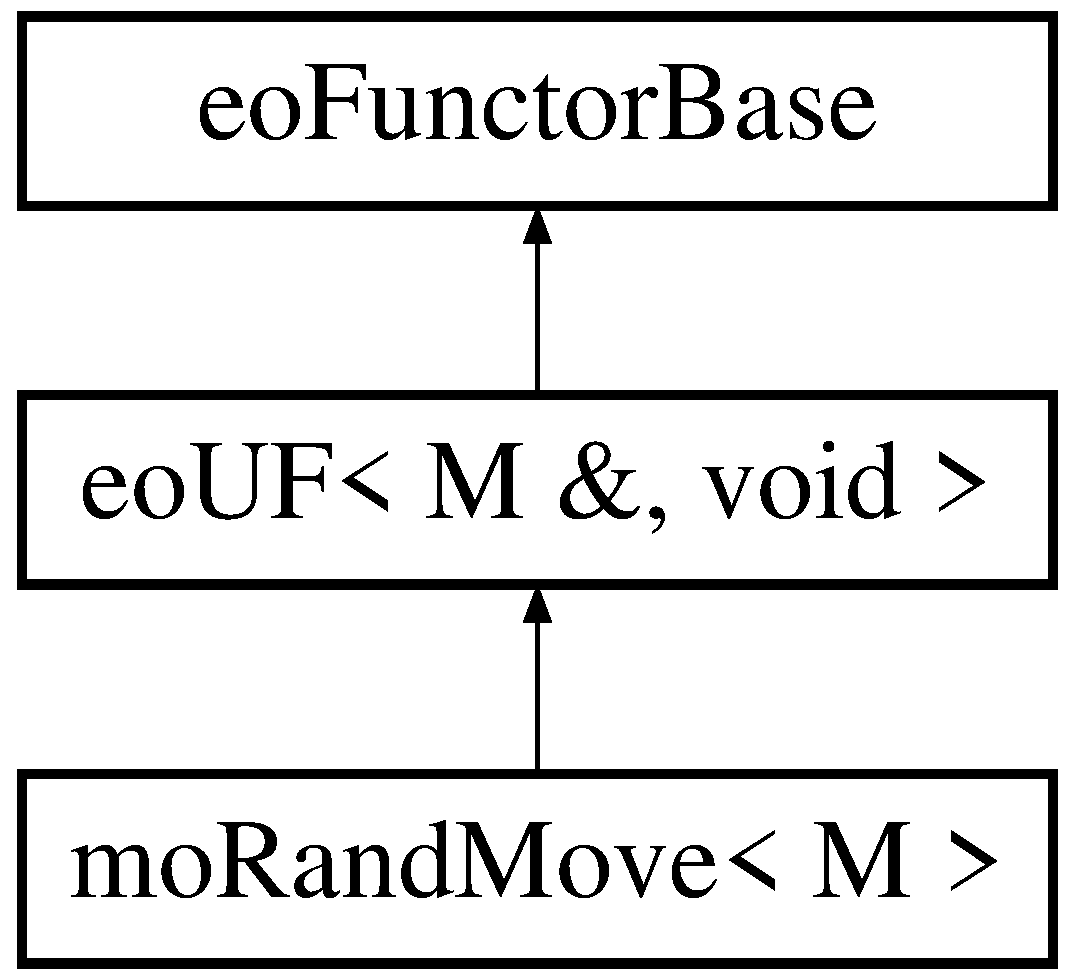
\includegraphics[height=3cm]{classmo_rand_move}
\end{center}
\end{figure}


\subsection{Detailed Description}
\subsubsection*{template$<$class M$>$ class moRandMove$<$ M $>$}

Random move generator. 

Only a description... An object that herits from this class needs to be designed in order to use a \doxyref{moSA}{p.}{classmo_s_a}. 



Definition at line 21 of file moRandMove.h.

The documentation for this class was generated from the following file:\begin{CompactItemize}
\item 
moRandMove.h\end{CompactItemize}

\section{mo\-SA$<$ M $>$ Class Template Reference}
\label{classmo_s_a}\index{moSA@{moSA}}
Simulated Annealing (SA).  


{\tt \#include $<$mo\-SA.h$>$}

Inheritance diagram for mo\-SA$<$ M $>$::\begin{figure}[H]
\begin{center}
\leavevmode
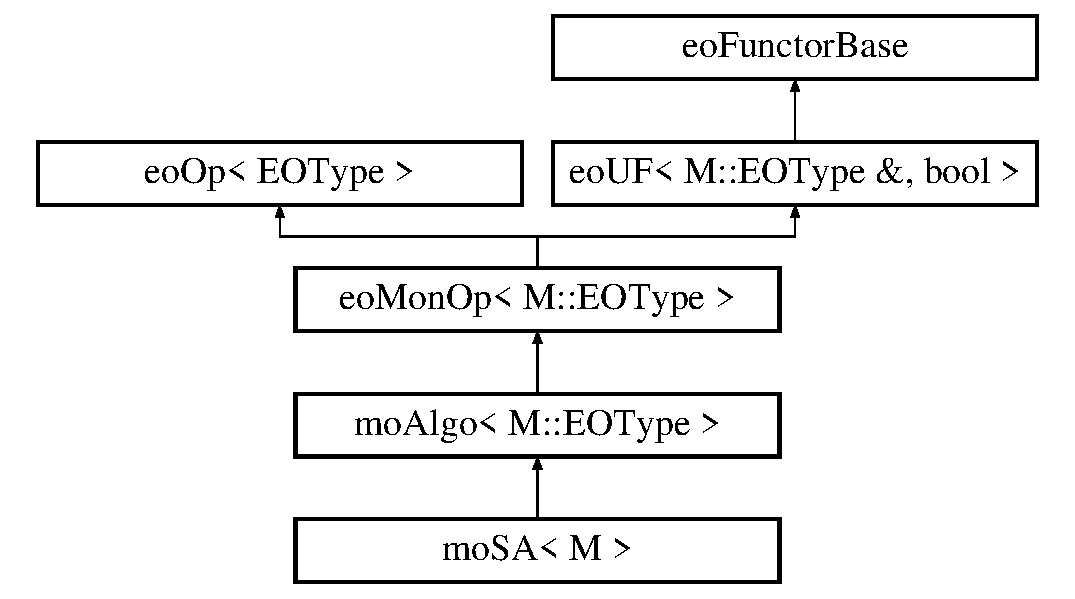
\includegraphics[height=5cm]{classmo_s_a}
\end{center}
\end{figure}
\subsection*{Public Member Functions}
\begin{CompactItemize}
\item 
{\bf mo\-SA} ({\bf mo\-Rand\-Move}$<$ M $>$ \&\_\-\_\-move\_\-rand, {\bf mo\-Move\-Incr\-Eval}$<$ M $>$ \&\_\-\_\-incr\_\-eval, {\bf mo\-Sol\-Continue}$<$ {\bf EOT} $>$ \&\_\-\_\-cont, double \_\-\_\-init\_\-temp, {\bf mo\-Cool\-Sched} \&\_\-\_\-cool\_\-sched, {\bf eo\-Eval\-Func}$<$ {\bf EOT} $>$ \&\_\-\_\-full\_\-eval)
\begin{CompactList}\small\item\em SA constructor. \item\end{CompactList}\item 
bool {\bf operator()} ({\bf EOT} \&\_\-\_\-sol)
\begin{CompactList}\small\item\em function that launches the SA algorithm. \item\end{CompactList}\end{CompactItemize}
\subsection*{Private Types}
\begin{CompactItemize}
\item 
typedef M::EOType {\bf EOT}\label{classmo_s_a_d5d64a8797bdedc7b3af7893aded0bd5}

\begin{CompactList}\small\item\em Alias for the type. \item\end{CompactList}\item 
typedef EOT::Fitness {\bf Fitness}\label{classmo_s_a_97f1a40d5ab5a0b3f878d0347b34804b}

\begin{CompactList}\small\item\em Alias for the fitness. \item\end{CompactList}\end{CompactItemize}
\subsection*{Private Attributes}
\begin{CompactItemize}
\item 
{\bf mo\-Rand\-Move}$<$ M $>$ \& {\bf move\_\-rand}\label{classmo_s_a_71c49935b63a202d25888a5f86121fec}

\begin{CompactList}\small\item\em A move generator (generally randomly). \item\end{CompactList}\item 
{\bf mo\-Move\-Incr\-Eval}$<$ M $>$ \& {\bf incr\_\-eval}\label{classmo_s_a_4c3be32e9832e465b24e6d33559356bc}

\begin{CompactList}\small\item\em A (generally) efficient evaluation function. \item\end{CompactList}\item 
{\bf mo\-Sol\-Continue}$<$ {\bf EOT} $>$ \& {\bf cont}\label{classmo_s_a_54484c8a514866ea496e0058c2e09716}

\begin{CompactList}\small\item\em Stopping criterion before temperature update. \item\end{CompactList}\item 
double {\bf init\_\-temp}\label{classmo_s_a_f1af7636b52aa5f6b381f8187b667bd4}

\begin{CompactList}\small\item\em Initial temperature. \item\end{CompactList}\item 
{\bf mo\-Cool\-Sched} \& {\bf cool\_\-sched}\label{classmo_s_a_c7aaf7424aa1b9f889d2ba9c959e5a1d}

\begin{CompactList}\small\item\em The cooling schedule. \item\end{CompactList}\item 
{\bf eo\-Eval\-Func}$<$ {\bf EOT} $>$ \& {\bf full\_\-eval}\label{classmo_s_a_bcd6a940046f23dd741444c0b85edf2c}

\begin{CompactList}\small\item\em A full evaluation function. \item\end{CompactList}\end{CompactItemize}


\subsection{Detailed Description}
\subsubsection*{template$<$class M$>$ class mo\-SA$<$ M $>$}

Simulated Annealing (SA). 

Class that describes a Simulated Annealing algorithm. 



Definition at line 32 of file mo\-SA.h.

\subsection{Constructor \& Destructor Documentation}
\index{moSA@{mo\-SA}!moSA@{moSA}}
\index{moSA@{moSA}!moSA@{mo\-SA}}
\subsubsection{\setlength{\rightskip}{0pt plus 5cm}template$<$class M$>$ {\bf mo\-SA}$<$ M $>$::{\bf mo\-SA} ({\bf mo\-Rand\-Move}$<$ M $>$ \& {\em \_\-\_\-move\_\-rand}, {\bf mo\-Move\-Incr\-Eval}$<$ M $>$ \& {\em \_\-\_\-incr\_\-eval}, {\bf mo\-Sol\-Continue}$<$ {\bf EOT} $>$ \& {\em \_\-\_\-cont}, double {\em \_\-\_\-init\_\-temp}, {\bf mo\-Cool\-Sched} \& {\em \_\-\_\-cool\_\-sched}, {\bf eo\-Eval\-Func}$<$ {\bf EOT} $>$ \& {\em \_\-\_\-full\_\-eval})\hspace{0.3cm}{\tt  [inline]}}\label{classmo_s_a_ef9ffb0d95c599e0a06c78db5f2f4b12}


SA constructor. 

All the boxes used by a SA need to be given.

\begin{Desc}
\item[Parameters:]
\begin{description}
\item[{\em \_\-\_\-move\_\-rand}]a move generator (generally randomly). \item[{\em \_\-\_\-incr\_\-eval}]a (generaly) efficient evaluation function \item[{\em \_\-\_\-cont}]a stopping criterion. \item[{\em \_\-\_\-init\_\-temp}]the initial temperature. \item[{\em \_\-\_\-cool\_\-sched}]a cooling schedule, describes how the temperature is modified. \item[{\em \_\-\_\-full\_\-eval}]a full evaluation function. \end{description}
\end{Desc}


Definition at line 60 of file mo\-SA.h.

\subsection{Member Function Documentation}
\index{moSA@{mo\-SA}!operator()@{operator()}}
\index{operator()@{operator()}!moSA@{mo\-SA}}
\subsubsection{\setlength{\rightskip}{0pt plus 5cm}template$<$class M$>$ bool {\bf mo\-SA}$<$ M $>$::operator() ({\bf EOT} \& {\em \_\-\_\-sol})\hspace{0.3cm}{\tt  [inline, virtual]}}\label{classmo_s_a_0e4c54b57bc13fcbd4763883b8f719e5}


function that launches the SA algorithm. 

As a \doxyref{mo\-TS}{p.}{classmo_t_s} or a \doxyref{mo\-HC}{p.}{classmo_h_c}, the SA can be used for HYBRIDATION in an evolutionary algorithm.

\begin{Desc}
\item[Parameters:]
\begin{description}
\item[{\em \_\-\_\-sol}]a solution to improve. \end{description}
\end{Desc}
\begin{Desc}
\item[Returns:]TRUE. \end{Desc}


Implements {\bf eo\-UF$<$ M::EOType \&, bool $>$}.

Definition at line 82 of file mo\-SA.h.

References mo\-SA$<$ M $>$::cont, mo\-SA$<$ M $>$::cool\_\-sched, mo\-SA$<$ M $>$::full\_\-eval, mo\-SA$<$ M $>$::incr\_\-eval, mo\-SA$<$ M $>$::init\_\-temp, and mo\-SA$<$ M $>$::move\_\-rand.

The documentation for this class was generated from the following file:\begin{CompactItemize}
\item 
mo\-SA.h\end{CompactItemize}

\section{mo\-Simple\-Move\-Tabu\-List$<$ M $>$ Class Template Reference}
\label{classmo_simple_move_tabu_list}\index{moSimpleMoveTabuList@{moSimpleMoveTabuList}}
Class describing a move tabu list with a limited memory.  


{\tt \#include $<$mo\-Simple\-Move\-Tabu\-List.h$>$}

Inheritance diagram for mo\-Simple\-Move\-Tabu\-List$<$ M $>$::\begin{figure}[H]
\begin{center}
\leavevmode
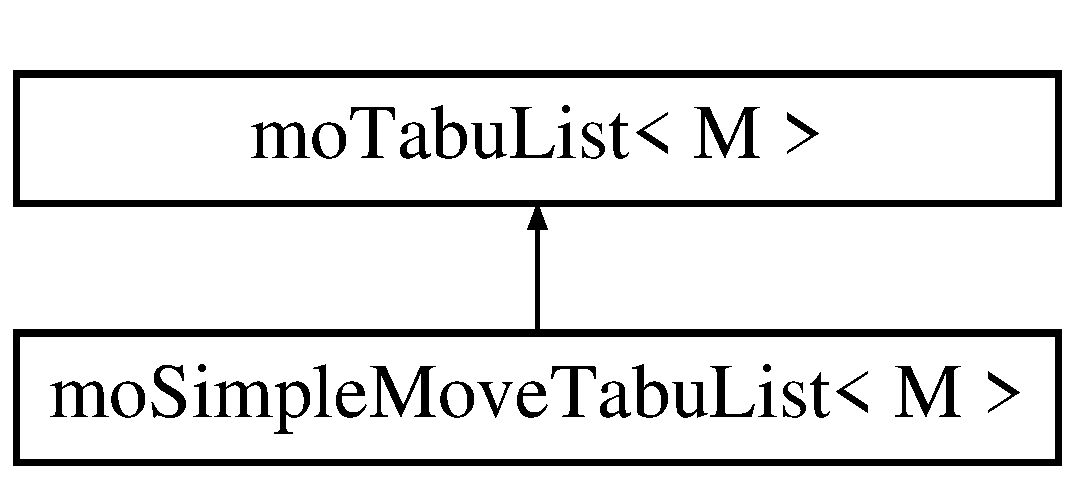
\includegraphics[height=4cm]{classmo_simple_move_tabu_list}
\end{center}
\end{figure}
\subsection*{Public Types}
\begin{CompactItemize}
\item 
typedef M::EOType {\bf EOT}\label{classmo_simple_move_tabu_list_91286ff3ba6b1e9e1db9e4fdade2edb7}

\begin{CompactList}\small\item\em Alias for the type. \item\end{CompactList}\end{CompactItemize}
\subsection*{Public Member Functions}
\begin{CompactItemize}
\item 
{\bf mo\-Simple\-Move\-Tabu\-List} (unsigned \_\-\_\-size)\label{classmo_simple_move_tabu_list_d29bb1cfc8d1fd2de1cccf821d066b66}

\begin{CompactList}\small\item\em Constructor. \item\end{CompactList}\item 
bool {\bf operator()} (const M \&\_\-\_\-move, const {\bf EOT} \&\_\-\_\-sol)
\begin{CompactList}\small\item\em Function that indicates if, in a given state, the \_\-move is tabu or not. \item\end{CompactList}\item 
void {\bf add} (const M \&\_\-\_\-move, const {\bf EOT} \&\_\-\_\-sol)
\begin{CompactList}\small\item\em Procedure to add a move in the tabu list. \item\end{CompactList}\item 
void {\bf update} ()
\begin{CompactList}\small\item\em Procedure that updates the tabu list content. \item\end{CompactList}\item 
void {\bf init} ()
\begin{CompactList}\small\item\em Procedure which initialises the tabu list. \item\end{CompactList}\end{CompactItemize}
\subsection*{Private Member Functions}
\begin{CompactItemize}
\item 
void {\bf remove\-Move} (const M \&\_\-\_\-move)
\begin{CompactList}\small\item\em Procedure that removes a given move from the tabu list (if it is into, else do nothing). \item\end{CompactList}\end{CompactItemize}
\subsection*{Private Attributes}
\begin{CompactItemize}
\item 
unsigned {\bf max\-Size}\label{classmo_simple_move_tabu_list_9f4860b378366e774c61a0d2034811e1}

\begin{CompactList}\small\item\em The maximum size of the tabu list. \item\end{CompactList}\item 
unsigned {\bf current\-Size}\label{classmo_simple_move_tabu_list_bd417b084e01343cba914a8193dab3a1}

\begin{CompactList}\small\item\em The current size of the tabu list. \item\end{CompactList}\item 
std::list$<$ M $>$ {\bf tabu\-List}\label{classmo_simple_move_tabu_list_d91bc838361524720616b44eda9b2c3a}

\begin{CompactList}\small\item\em The move tabu list. \item\end{CompactList}\end{CompactItemize}


\subsection{Detailed Description}
\subsubsection*{template$<$class M$>$ class mo\-Simple\-Move\-Tabu\-List$<$ M $>$}

Class describing a move tabu list with a limited memory. 



Definition at line 22 of file mo\-Simple\-Move\-Tabu\-List.h.

\subsection{Member Function Documentation}
\index{moSimpleMoveTabuList@{mo\-Simple\-Move\-Tabu\-List}!operator()@{operator()}}
\index{operator()@{operator()}!moSimpleMoveTabuList@{mo\-Simple\-Move\-Tabu\-List}}
\subsubsection{\setlength{\rightskip}{0pt plus 5cm}template$<$class M$>$ bool {\bf mo\-Simple\-Move\-Tabu\-List}$<$ M $>$::operator() (const M \& {\em \_\-\_\-move}, const {\bf EOT} \& {\em \_\-\_\-sol})\hspace{0.3cm}{\tt  [inline]}}\label{classmo_simple_move_tabu_list_bb7fe9da28617f56734af71c42c8265a}


Function that indicates if, in a given state, the \_\-move is tabu or not. 

\begin{Desc}
\item[Parameters:]
\begin{description}
\item[{\em \_\-\_\-move}]A given \doxyref{mo\-Move}{p.}{classmo_move}. \item[{\em \_\-\_\-sol}]A solution. \end{description}
\end{Desc}
\begin{Desc}
\item[Returns:]true or false. \end{Desc}


Definition at line 46 of file mo\-Simple\-Move\-Tabu\-List.h.

References mo\-Simple\-Move\-Tabu\-List$<$ M $>$::tabu\-List.\index{moSimpleMoveTabuList@{mo\-Simple\-Move\-Tabu\-List}!add@{add}}
\index{add@{add}!moSimpleMoveTabuList@{mo\-Simple\-Move\-Tabu\-List}}
\subsubsection{\setlength{\rightskip}{0pt plus 5cm}template$<$class M$>$ void {\bf mo\-Simple\-Move\-Tabu\-List}$<$ M $>$::add (const M \& {\em \_\-\_\-move}, const {\bf EOT} \& {\em \_\-\_\-sol})\hspace{0.3cm}{\tt  [inline, virtual]}}\label{classmo_simple_move_tabu_list_43c979a9ec876c5e5b591b1c422395ef}


Procedure to add a move in the tabu list. 

The two parameters have not to be modified so they are constant parameters.

\begin{Desc}
\item[Parameters:]
\begin{description}
\item[{\em \_\-\_\-move}]a new tabu move. \item[{\em \_\-\_\-sol}]the origianl solution associated to this move. \end{description}
\end{Desc}


Implements {\bf mo\-Tabu\-List$<$ M $>$} \doxyref{}{p.}{classmo_tabu_list_d279d72cb486d812da1ad3d24a69c286}.

Definition at line 60 of file mo\-Simple\-Move\-Tabu\-List.h.

References mo\-Simple\-Move\-Tabu\-List$<$ M $>$::current\-Size, mo\-Simple\-Move\-Tabu\-List$<$ M $>$::max\-Size, mo\-Simple\-Move\-Tabu\-List$<$ M $>$::remove\-Move(), and mo\-Simple\-Move\-Tabu\-List$<$ M $>$::tabu\-List.\index{moSimpleMoveTabuList@{mo\-Simple\-Move\-Tabu\-List}!update@{update}}
\index{update@{update}!moSimpleMoveTabuList@{mo\-Simple\-Move\-Tabu\-List}}
\subsubsection{\setlength{\rightskip}{0pt plus 5cm}template$<$class M$>$ void {\bf mo\-Simple\-Move\-Tabu\-List}$<$ M $>$::update ()\hspace{0.3cm}{\tt  [inline, virtual]}}\label{classmo_simple_move_tabu_list_96cffc8118456ed762b07b9fc0e0679f}


Procedure that updates the tabu list content. 

Generally, a counter associated to each saved move is decreased by one. 

Implements {\bf mo\-Tabu\-List$<$ M $>$} \doxyref{}{p.}{classmo_tabu_list_a2e5d1132f064093c8ed57046405f5ca}.

Definition at line 82 of file mo\-Simple\-Move\-Tabu\-List.h.\index{moSimpleMoveTabuList@{mo\-Simple\-Move\-Tabu\-List}!init@{init}}
\index{init@{init}!moSimpleMoveTabuList@{mo\-Simple\-Move\-Tabu\-List}}
\subsubsection{\setlength{\rightskip}{0pt plus 5cm}template$<$class M$>$ void {\bf mo\-Simple\-Move\-Tabu\-List}$<$ M $>$::init ()\hspace{0.3cm}{\tt  [inline, virtual]}}\label{classmo_simple_move_tabu_list_b91ae9971be30769757d1ad92c6009dc}


Procedure which initialises the tabu list. 

Can be useful if the data structure needs to be allocated before being used. 

Implements {\bf mo\-Tabu\-List$<$ M $>$} \doxyref{}{p.}{classmo_tabu_list_0a06c459d56e8e2b408a8f3c6aec4e57}.

Definition at line 88 of file mo\-Simple\-Move\-Tabu\-List.h.\index{moSimpleMoveTabuList@{mo\-Simple\-Move\-Tabu\-List}!removeMove@{removeMove}}
\index{removeMove@{removeMove}!moSimpleMoveTabuList@{mo\-Simple\-Move\-Tabu\-List}}
\subsubsection{\setlength{\rightskip}{0pt plus 5cm}template$<$class M$>$ void {\bf mo\-Simple\-Move\-Tabu\-List}$<$ M $>$::remove\-Move (const M \& {\em \_\-\_\-move})\hspace{0.3cm}{\tt  [inline, private]}}\label{classmo_simple_move_tabu_list_a3fa2bd19e09f1541878fa28e867d20f}


Procedure that removes a given move from the tabu list (if it is into, else do nothing). 

\begin{Desc}
\item[Parameters:]
\begin{description}
\item[{\em \_\-\_\-move}]A given \doxyref{mo\-Move}{p.}{classmo_move}. \end{description}
\end{Desc}


Definition at line 100 of file mo\-Simple\-Move\-Tabu\-List.h.

References mo\-Simple\-Move\-Tabu\-List$<$ M $>$::tabu\-List.

Referenced by mo\-Simple\-Move\-Tabu\-List$<$ M $>$::add().

The documentation for this class was generated from the following file:\begin{CompactItemize}
\item 
mo\-Simple\-Move\-Tabu\-List.h\end{CompactItemize}

\section{mo\-Simple\-Solution\-Tabu\-List$<$ M $>$ Class Template Reference}
\label{classmo_simple_solution_tabu_list}\index{moSimpleSolutionTabuList@{moSimpleSolutionTabuList}}
Class describing a solution tabu list with limited length.  


{\tt \#include $<$mo\-Simple\-Solution\-Tabu\-List.h$>$}

Inheritance diagram for mo\-Simple\-Solution\-Tabu\-List$<$ M $>$::\begin{figure}[H]
\begin{center}
\leavevmode
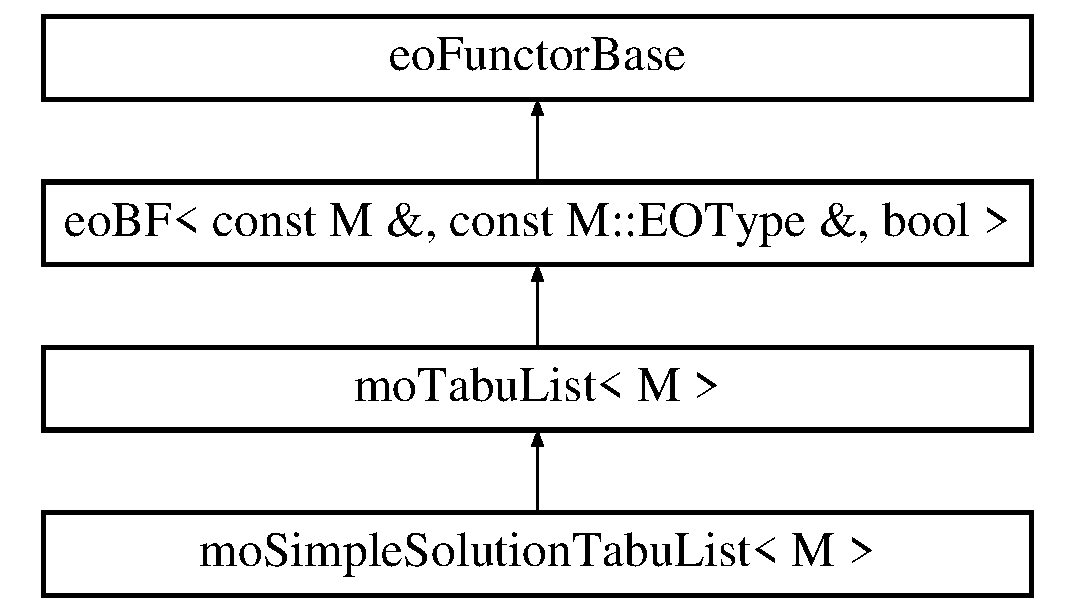
\includegraphics[height=2cm]{classmo_simple_solution_tabu_list}
\end{center}
\end{figure}
\subsection*{Public Types}
\begin{CompactItemize}
\item 
typedef M::EOType \bf{EOT}\label{classmo_simple_solution_tabu_list_881060871a6b49e5e8554c5df85176d9}

\begin{CompactList}\small\item\em Alias for the type. \item\end{CompactList}\item 
typedef std::list$<$ \bf{EOT} $>$::iterator \bf{solution\-Iterator}\label{classmo_simple_solution_tabu_list_3438db9ed9e1a94a24c418d8cbadec54}

\begin{CompactList}\small\item\em Alias for an iterator of a solution list. \item\end{CompactList}\end{CompactItemize}
\subsection*{Public Member Functions}
\begin{CompactItemize}
\item 
\bf{mo\-Simple\-Solution\-Tabu\-List} (unsigned int \_\-memory\_\-maximum\_\-size)
\begin{CompactList}\small\item\em Constructor. \item\end{CompactList}\item 
bool \bf{operator()} (const M \&\_\-move, const \bf{EOT} \&\_\-solution)
\begin{CompactList}\small\item\em Function that indicates if, in a given state, the \_\-move is tabu or not. \item\end{CompactList}\item 
void \bf{add} (const M \&\_\-move, const \bf{EOT} \&\_\-solution)
\begin{CompactList}\small\item\em Procedure to add a move in the tabu list. \item\end{CompactList}\item 
void \bf{update} ()
\begin{CompactList}\small\item\em Procedure that updates the tabu list content. \item\end{CompactList}\item 
void \bf{init} ()
\begin{CompactList}\small\item\em Procedure which initialises the tabu list. \item\end{CompactList}\end{CompactItemize}
\subsection*{Private Member Functions}
\begin{CompactItemize}
\item 
void \bf{remove\-Solution} (const \bf{EOT} \&\_\-solution)
\begin{CompactList}\small\item\em Procedure that removes a given solution from the tabu list (if it is into, else does nothing). \item\end{CompactList}\end{CompactItemize}
\subsection*{Private Attributes}
\begin{CompactItemize}
\item 
unsigned int \bf{memory\_\-maximum\_\-size}\label{classmo_simple_solution_tabu_list_06631e7b9a2511e3c11540aa14b9e636}

\begin{CompactList}\small\item\em The maximum size of the tabu list. \item\end{CompactList}\item 
unsigned int \bf{memory\_\-size}\label{classmo_simple_solution_tabu_list_0d54e6b0af0e6088aafae596392c9490}

\begin{CompactList}\small\item\em The current size of the tabu list. \item\end{CompactList}\item 
std::list$<$ \bf{EOT} $>$ \bf{tabu\-List}\label{classmo_simple_solution_tabu_list_75df9cd683528d3722d02bac407b710b}

\begin{CompactList}\small\item\em The solution tabu list. \item\end{CompactList}\end{CompactItemize}


\subsection{Detailed Description}
\subsubsection*{template$<$class M$>$ class mo\-Simple\-Solution\-Tabu\-List$<$ M $>$}

Class describing a solution tabu list with limited length. 



Definition at line 46 of file mo\-Simple\-Solution\-Tabu\-List.h.

\subsection{Constructor \& Destructor Documentation}
\index{moSimpleSolutionTabuList@{mo\-Simple\-Solution\-Tabu\-List}!moSimpleSolutionTabuList@{moSimpleSolutionTabuList}}
\index{moSimpleSolutionTabuList@{moSimpleSolutionTabuList}!moSimpleSolutionTabuList@{mo\-Simple\-Solution\-Tabu\-List}}
\subsubsection{\setlength{\rightskip}{0pt plus 5cm}template$<$class M$>$ \bf{mo\-Simple\-Solution\-Tabu\-List}$<$ M $>$::\bf{mo\-Simple\-Solution\-Tabu\-List} (unsigned int {\em \_\-memory\_\-maximum\_\-size})\hspace{0.3cm}{\tt  [inline]}}\label{classmo_simple_solution_tabu_list_8499bf947de47519d155e9e45f815d41}


Constructor. 

\begin{Desc}
\item[Parameters:]
\begin{description}
\item[{\em \_\-memory\_\-maximum\_\-size}]The maximum size of the solution tabu list. \end{description}
\end{Desc}


Definition at line 60 of file mo\-Simple\-Solution\-Tabu\-List.h.

\subsection{Member Function Documentation}
\index{moSimpleSolutionTabuList@{mo\-Simple\-Solution\-Tabu\-List}!operator()@{operator()}}
\index{operator()@{operator()}!moSimpleSolutionTabuList@{mo\-Simple\-Solution\-Tabu\-List}}
\subsubsection{\setlength{\rightskip}{0pt plus 5cm}template$<$class M$>$ bool \bf{mo\-Simple\-Solution\-Tabu\-List}$<$ M $>$::operator() (const M \& {\em \_\-move}, const \bf{EOT} \& {\em \_\-solution})\hspace{0.3cm}{\tt  [inline]}}\label{classmo_simple_solution_tabu_list_9052858ae3e6765cbe4c344bdae6c692}


Function that indicates if, in a given state, the \_\-move is tabu or not. 

\begin{Desc}
\item[Parameters:]
\begin{description}
\item[{\em \_\-move}]A given \doxyref{mo\-Move}{p.}{classmo_move}. \item[{\em \_\-solution}]A solution. \end{description}
\end{Desc}
\begin{Desc}
\item[Returns:]true or false. \end{Desc}


Definition at line 69 of file mo\-Simple\-Solution\-Tabu\-List.h.

References mo\-Simple\-Solution\-Tabu\-List$<$ M $>$::tabu\-List.\index{moSimpleSolutionTabuList@{mo\-Simple\-Solution\-Tabu\-List}!add@{add}}
\index{add@{add}!moSimpleSolutionTabuList@{mo\-Simple\-Solution\-Tabu\-List}}
\subsubsection{\setlength{\rightskip}{0pt plus 5cm}template$<$class M$>$ void \bf{mo\-Simple\-Solution\-Tabu\-List}$<$ M $>$::add (const M \& {\em \_\-move}, const \bf{EOT} \& {\em \_\-solution})\hspace{0.3cm}{\tt  [inline, virtual]}}\label{classmo_simple_solution_tabu_list_58ae13e7642c429ea51ff679a932aceb}


Procedure to add a move in the tabu list. 

The two parameters have not to be modified so they are constant parameters.

\begin{Desc}
\item[Parameters:]
\begin{description}
\item[{\em \_\-move}]a new tabu move. \item[{\em \_\-solution}]the origianl solution associated to this move. \end{description}
\end{Desc}


Implements \bf{mo\-Tabu\-List$<$ M $>$} \doxyref{p.}{classmo_tabu_list_55204939b6d67b6d37b4af725d70cf6d}.

Definition at line 89 of file mo\-Simple\-Solution\-Tabu\-List.h.

References mo\-Simple\-Solution\-Tabu\-List$<$ M $>$::memory\_\-maximum\_\-size, mo\-Simple\-Solution\-Tabu\-List$<$ M $>$::memory\_\-size, mo\-Simple\-Solution\-Tabu\-List$<$ M $>$::remove\-Solution(), and mo\-Simple\-Solution\-Tabu\-List$<$ M $>$::tabu\-List.\index{moSimpleSolutionTabuList@{mo\-Simple\-Solution\-Tabu\-List}!update@{update}}
\index{update@{update}!moSimpleSolutionTabuList@{mo\-Simple\-Solution\-Tabu\-List}}
\subsubsection{\setlength{\rightskip}{0pt plus 5cm}template$<$class M$>$ void \bf{mo\-Simple\-Solution\-Tabu\-List}$<$ M $>$::update ()\hspace{0.3cm}{\tt  [inline, virtual]}}\label{classmo_simple_solution_tabu_list_91b8b01dba7ffea8b63765d931e56f56}


Procedure that updates the tabu list content. 

Generally, a counter associated to each saved move is decreased by one. 

Implements \bf{mo\-Tabu\-List$<$ M $>$} \doxyref{p.}{classmo_tabu_list_a2e5d1132f064093c8ed57046405f5ca}.

Definition at line 115 of file mo\-Simple\-Solution\-Tabu\-List.h.\index{moSimpleSolutionTabuList@{mo\-Simple\-Solution\-Tabu\-List}!init@{init}}
\index{init@{init}!moSimpleSolutionTabuList@{mo\-Simple\-Solution\-Tabu\-List}}
\subsubsection{\setlength{\rightskip}{0pt plus 5cm}template$<$class M$>$ void \bf{mo\-Simple\-Solution\-Tabu\-List}$<$ M $>$::init ()\hspace{0.3cm}{\tt  [inline, virtual]}}\label{classmo_simple_solution_tabu_list_d5645c39fec71a6110a2cbccbb08b816}


Procedure which initialises the tabu list. 

Can be useful if the data structure needs to be allocated before being used. 

Implements \bf{mo\-Tabu\-List$<$ M $>$} \doxyref{p.}{classmo_tabu_list_0a06c459d56e8e2b408a8f3c6aec4e57}.

Definition at line 120 of file mo\-Simple\-Solution\-Tabu\-List.h.\index{moSimpleSolutionTabuList@{mo\-Simple\-Solution\-Tabu\-List}!removeSolution@{removeSolution}}
\index{removeSolution@{removeSolution}!moSimpleSolutionTabuList@{mo\-Simple\-Solution\-Tabu\-List}}
\subsubsection{\setlength{\rightskip}{0pt plus 5cm}template$<$class M$>$ void \bf{mo\-Simple\-Solution\-Tabu\-List}$<$ M $>$::remove\-Solution (const \bf{EOT} \& {\em \_\-solution})\hspace{0.3cm}{\tt  [inline, private]}}\label{classmo_simple_solution_tabu_list_e4a57001a201e1fb7446902381a7ac7d}


Procedure that removes a given solution from the tabu list (if it is into, else does nothing). 

\begin{Desc}
\item[Parameters:]
\begin{description}
\item[{\em \_\-solution}]A given solution. \end{description}
\end{Desc}


Definition at line 131 of file mo\-Simple\-Solution\-Tabu\-List.h.

References mo\-Simple\-Solution\-Tabu\-List$<$ M $>$::tabu\-List.

Referenced by mo\-Simple\-Solution\-Tabu\-List$<$ M $>$::add().

The documentation for this class was generated from the following file:\begin{CompactItemize}
\item 
mo\-Simple\-Solution\-Tabu\-List.h\end{CompactItemize}

\section{moSolContinue$<$ EOT $>$ Class Template Reference}
\label{classmo_sol_continue}\index{moSolContinue@{moSolContinue}}
Class that describes a stopping criterion for a solution-based heuristic.  


{\tt \#include $<$moSolContinue.h$>$}

Inheritance diagram for moSolContinue$<$ EOT $>$::\begin{figure}[H]
\begin{center}
\leavevmode
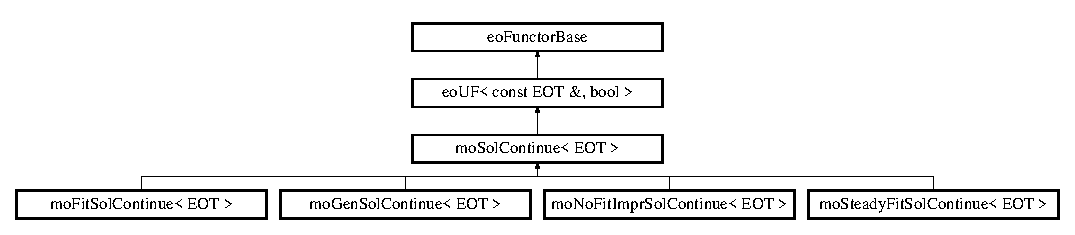
\includegraphics[height=2.70531cm]{classmo_sol_continue}
\end{center}
\end{figure}
\subsection*{Public Member Functions}
\begin{CompactItemize}
\item 
virtual void {\bf init} ()=0
\begin{CompactList}\small\item\em Procedure which initialises all that the stopping criterion needs. \item\end{CompactList}\end{CompactItemize}


\subsection{Detailed Description}
\subsubsection*{template$<$class EOT$>$ class moSolContinue$<$ EOT $>$}

Class that describes a stopping criterion for a solution-based heuristic. 

It allows to add an initialisation procedure to an object that is a unary function ({\bf eoUF}). 



Definition at line 22 of file moSolContinue.h.

\subsection{Member Function Documentation}
\index{moSolContinue@{moSolContinue}!init@{init}}
\index{init@{init}!moSolContinue@{moSolContinue}}
\subsubsection{\setlength{\rightskip}{0pt plus 5cm}template$<$class EOT$>$ virtual void {\bf moSolContinue}$<$ EOT $>$::init ()\hspace{0.3cm}{\tt  [pure virtual]}}\label{classmo_sol_continue_064dc966a210f4ffb9515be3f03ca4c7}


Procedure which initialises all that the stopping criterion needs. 

Generally, it allocates some data structures or initialises some counters. 

Implemented in {\bf moFitSolContinue$<$ EOT $>$} \doxyref{}{p.}{classmo_fit_sol_continue_670bd895b4edfcd3aebb40d2295d7f7c}, {\bf moGenSolContinue$<$ EOT $>$} \doxyref{}{p.}{classmo_gen_sol_continue_6c5db8182157584b56507cc9075602d4}, {\bf moNoFitImprSolContinue$<$ EOT $>$} \doxyref{}{p.}{classmo_no_fit_impr_sol_continue_21641c0a38a4501baae6133cbc591de4}, and {\bf moSteadyFitSolContinue$<$ EOT $>$} \doxyref{}{p.}{classmo_steady_fit_sol_continue_87563493addc8e4b58982c55a67179b9}.

The documentation for this class was generated from the following file:\begin{CompactItemize}
\item 
moSolContinue.h\end{CompactItemize}

\section{moTabuList$<$ M $>$ Class Template Reference}
\label{classmo_tabu_list}\index{moTabuList@{moTabuList}}
Class describing a tabu list that a \doxyref{moTS}{p.}{classmo_t_s} uses.  


{\tt \#include $<$moTabuList.h$>$}

Inheritance diagram for moTabuList$<$ M $>$::\begin{figure}[H]
\begin{center}
\leavevmode
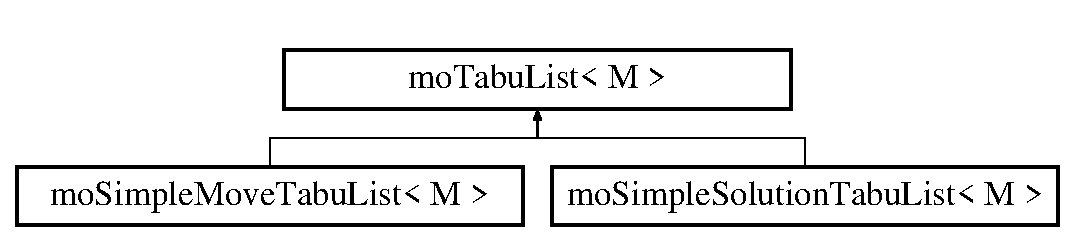
\includegraphics[height=3.88889cm]{classmo_tabu_list}
\end{center}
\end{figure}
\subsection*{Public Types}
\begin{CompactItemize}
\item 
typedef M::EOType {\bf EOT}\label{classmo_tabu_list_e219715cc3fdd5626764bc50ce6357df}

\begin{CompactList}\small\item\em Alias for the type. \item\end{CompactList}\end{CompactItemize}
\subsection*{Public Member Functions}
\begin{CompactItemize}
\item 
virtual void {\bf add} (const M \&\_\-\_\-move, const {\bf EOT} \&\_\-\_\-sol)=0
\begin{CompactList}\small\item\em Procedure to add a move in the tabu list. \item\end{CompactList}\item 
virtual void {\bf update} ()=0
\begin{CompactList}\small\item\em Procedure that updates the tabu list content. \item\end{CompactList}\item 
virtual void {\bf init} ()=0
\begin{CompactList}\small\item\em Procedure which initialises the tabu list. \item\end{CompactList}\end{CompactItemize}


\subsection{Detailed Description}
\subsubsection*{template$<$class M$>$ class moTabuList$<$ M $>$}

Class describing a tabu list that a \doxyref{moTS}{p.}{classmo_t_s} uses. 

It is only a description, does nothing... A new object that herits from this class has to be defined in order to be used in a \doxyref{moTS}{p.}{classmo_t_s}. 



Definition at line 45 of file moTabuList.h.

\subsection{Member Function Documentation}
\index{moTabuList@{moTabuList}!add@{add}}
\index{add@{add}!moTabuList@{moTabuList}}
\subsubsection{\setlength{\rightskip}{0pt plus 5cm}template$<$class M$>$ virtual void {\bf moTabuList}$<$ M $>$::add (const M \& {\em \_\-\_\-move}, const {\bf EOT} \& {\em \_\-\_\-sol})\hspace{0.3cm}{\tt  [pure virtual]}}\label{classmo_tabu_list_d279d72cb486d812da1ad3d24a69c286}


Procedure to add a move in the tabu list. 

The two parameters have not to be modified so they are constant parameters.

\begin{Desc}
\item[Parameters:]
\begin{description}
\item[{\em \_\-\_\-move}]a new tabu move. \item[{\em \_\-\_\-sol}]the origianl solution associated to this move. \end{description}
\end{Desc}


Implemented in {\bf moSimpleMoveTabuList$<$ M $>$} \doxyref{}{p.}{classmo_simple_move_tabu_list_43c979a9ec876c5e5b591b1c422395ef}, and {\bf moSimpleSolutionTabuList$<$ M $>$} \doxyref{}{p.}{classmo_simple_solution_tabu_list_fd6b3a1764121169650c969bba895615}.\index{moTabuList@{moTabuList}!update@{update}}
\index{update@{update}!moTabuList@{moTabuList}}
\subsubsection{\setlength{\rightskip}{0pt plus 5cm}template$<$class M$>$ virtual void {\bf moTabuList}$<$ M $>$::update ()\hspace{0.3cm}{\tt  [pure virtual]}}\label{classmo_tabu_list_a2e5d1132f064093c8ed57046405f5ca}


Procedure that updates the tabu list content. 

Generally, a counter associated to each saved move is decreased by one. 

Implemented in {\bf moSimpleMoveTabuList$<$ M $>$} \doxyref{}{p.}{classmo_simple_move_tabu_list_96cffc8118456ed762b07b9fc0e0679f}, and {\bf moSimpleSolutionTabuList$<$ M $>$} \doxyref{}{p.}{classmo_simple_solution_tabu_list_91b8b01dba7ffea8b63765d931e56f56}.\index{moTabuList@{moTabuList}!init@{init}}
\index{init@{init}!moTabuList@{moTabuList}}
\subsubsection{\setlength{\rightskip}{0pt plus 5cm}template$<$class M$>$ virtual void {\bf moTabuList}$<$ M $>$::init ()\hspace{0.3cm}{\tt  [pure virtual]}}\label{classmo_tabu_list_0a06c459d56e8e2b408a8f3c6aec4e57}


Procedure which initialises the tabu list. 

Can be useful if the data structure needs to be allocated before being used. 

Implemented in {\bf moSimpleMoveTabuList$<$ M $>$} \doxyref{}{p.}{classmo_simple_move_tabu_list_b91ae9971be30769757d1ad92c6009dc}, and {\bf moSimpleSolutionTabuList$<$ M $>$} \doxyref{}{p.}{classmo_simple_solution_tabu_list_d5645c39fec71a6110a2cbccbb08b816}.

The documentation for this class was generated from the following file:\begin{CompactItemize}
\item 
moTabuList.h\end{CompactItemize}

\section{moTS$<$ M $>$ Class Template Reference}
\label{classmo_t_s}\index{moTS@{moTS}}
Tabu Search (TS).  


{\tt \#include $<$moTS.h$>$}

Inherits {\bf moAlgo$<$ M::EOType $>$}.

\subsection*{Public Member Functions}
\begin{CompactItemize}
\item 
{\bf moTS} ({\bf moMoveInit}$<$ M $>$ \&\_\-move\_\-initializer, {\bf moNextMove}$<$ M $>$ \&\_\-next\_\-move\_\-generator, {\bf moMoveIncrEval}$<$ M $>$ \&\_\-incremental\_\-evaluation, {\bf moTabuList}$<$ M $>$ \&\_\-tabu\_\-list, {\bf moAspirCrit}$<$ M $>$ \&\_\-aspiration\_\-criterion, {\bf moSolContinue}$<$ {\bf EOT} $>$ \&\_\-continue, {\bf eoEvalFunc}$<$ {\bf EOT} $>$ \&\_\-full\_\-evaluation)
\begin{CompactList}\small\item\em Constructor of a \doxyref{moTS}{p.}{classmo_t_s} specifying all the boxes. \item\end{CompactList}\item 
{\bf moTS} ({\bf moMoveExpl}$<$ M $>$ \&\_\-move\_\-explorer, {\bf moSolContinue}$<$ {\bf EOT} $>$ \&\_\-continue, {\bf eoEvalFunc}$<$ {\bf EOT} $>$ \&\_\-full\_\-evaluation)
\begin{CompactList}\small\item\em Constructor with less parameters. \item\end{CompactList}\item 
bool {\bf operator()} ({\bf EOT} \&\_\-solution)
\begin{CompactList}\small\item\em {\bf Function} which launchs the Tabu Search. \item\end{CompactList}\end{CompactItemize}
\subsection*{Private Types}
\begin{CompactItemize}
\item 
typedef M::EOType {\bf EOT}\label{classmo_t_s_90d19d468c12ab5bd796948ce1ce79b1}

\begin{CompactList}\small\item\em Alias for the type. \item\end{CompactList}\item 
typedef EOT::Fitness {\bf Fitness}\label{classmo_t_s_aa0eefbb17111422e495d1255f876fca}

\begin{CompactList}\small\item\em Alias for the fitness. \item\end{CompactList}\end{CompactItemize}
\subsection*{Private Attributes}
\begin{CompactItemize}
\item 
{\bf moMoveExpl}$<$ M $>$ \& {\bf move\_\-explorer}\label{classmo_t_s_9fd948a2c586f1991f5a1eee927af8a6}

\begin{CompactList}\small\item\em Neighborhood explorer. \item\end{CompactList}\item 
{\bf moSolContinue}$<$ {\bf EOT} $>$ \& {\bf continu}\label{classmo_t_s_962a37393faf5239e657388d375cd9b3}

\begin{CompactList}\small\item\em Stop criterion. \item\end{CompactList}\item 
{\bf eoEvalFunc}$<$ {\bf EOT} $>$ \& {\bf full\_\-evaluation}\label{classmo_t_s_f44bb408007e2bff99f7a201842e8e48}

\begin{CompactList}\small\item\em Full evaluation function. \item\end{CompactList}\end{CompactItemize}


\subsection{Detailed Description}
\subsubsection*{template$<$class M$>$ class moTS$<$ M $>$}

Tabu Search (TS). 

Generic algorithm that describes a tabu search. 

Definition at line 50 of file moTS.h.

\subsection{Constructor \& Destructor Documentation}
\index{moTS@{moTS}!moTS@{moTS}}
\index{moTS@{moTS}!moTS@{moTS}}
\subsubsection{\setlength{\rightskip}{0pt plus 5cm}template$<$class M$>$ {\bf moTS}$<$ M $>$::{\bf moTS} ({\bf moMoveInit}$<$ M $>$ \& {\em \_\-move\_\-initializer}, {\bf moNextMove}$<$ M $>$ \& {\em \_\-next\_\-move\_\-generator}, {\bf moMoveIncrEval}$<$ M $>$ \& {\em \_\-incremental\_\-evaluation}, {\bf moTabuList}$<$ M $>$ \& {\em \_\-tabu\_\-list}, {\bf moAspirCrit}$<$ M $>$ \& {\em \_\-aspiration\_\-criterion}, {\bf moSolContinue}$<$ {\bf EOT} $>$ \& {\em \_\-continue}, {\bf eoEvalFunc}$<$ {\bf EOT} $>$ \& {\em \_\-full\_\-evaluation})\hspace{0.3cm}{\tt  [inline]}}\label{classmo_t_s_336408ddf8b7a29ffa8e01e9c18d8e10}


Constructor of a \doxyref{moTS}{p.}{classmo_t_s} specifying all the boxes. 

In this constructor, a \doxyref{moTSMoveLoopExpl}{p.}{classmo_t_s_move_loop_expl} is instanciated.

\begin{Desc}
\item[Parameters:]
\begin{description}
\item[{\em \_\-move\_\-initializer}]The move initializer. \item[{\em \_\-next\_\-move\_\-generator}]The neighbourhood explorer. \item[{\em \_\-incremental\_\-evaluation}]The (generally) efficient evaluation. \item[{\em \_\-tabu\_\-list}]The tabu list. \item[{\em \_\-aspiration\_\-criterion}]An aspiration criterion. \item[{\em \_\-continue}]The stopping criterion. \item[{\em \_\-full\_\-evaluation}]A full evaluation function. \end{description}
\end{Desc}


Definition at line 72 of file moTS.h.\index{moTS@{moTS}!moTS@{moTS}}
\index{moTS@{moTS}!moTS@{moTS}}
\subsubsection{\setlength{\rightskip}{0pt plus 5cm}template$<$class M$>$ {\bf moTS}$<$ M $>$::{\bf moTS} ({\bf moMoveExpl}$<$ M $>$ \& {\em \_\-move\_\-explorer}, {\bf moSolContinue}$<$ {\bf EOT} $>$ \& {\em \_\-continue}, {\bf eoEvalFunc}$<$ {\bf EOT} $>$ \& {\em \_\-full\_\-evaluation})\hspace{0.3cm}{\tt  [inline]}}\label{classmo_t_s_7e435fac1b8d5a410b7374d114e005e2}


Constructor with less parameters. 

The explorer is given in the parameters.

\begin{Desc}
\item[Parameters:]
\begin{description}
\item[{\em \_\-move\_\-explorer}]The explorer (generally different that a \doxyref{moTSMoveLoopExpl}{p.}{classmo_t_s_move_loop_expl}). \item[{\em \_\-continue}]The stopping criterion. \item[{\em \_\-full\_\-evaluation}]A full evaluation function. \end{description}
\end{Desc}


Definition at line 89 of file moTS.h.

\subsection{Member Function Documentation}
\index{moTS@{moTS}!operator()@{operator()}}
\index{operator()@{operator()}!moTS@{moTS}}
\subsubsection{\setlength{\rightskip}{0pt plus 5cm}template$<$class M$>$ bool {\bf moTS}$<$ M $>$::operator() ({\bf EOT} \& {\em \_\-solution})\hspace{0.3cm}{\tt  [inline, virtual]}}\label{classmo_t_s_2a011779723e24a5132a37593775bf56}


{\bf Function} which launchs the Tabu Search. 

Algorithm of the tabu search. As a \doxyref{moSA}{p.}{classmo_s_a} or a \doxyref{moHC}{p.}{classmo_h_c}, it can be used for HYBRIDATION in an evolutionary algorithm. For security a lock (pthread\_\-mutex\_\-t) is closed during the algorithm.

\begin{Desc}
\item[Parameters:]
\begin{description}
\item[{\em \_\-solution}]a solution to improve. \end{description}
\end{Desc}
\begin{Desc}
\item[Returns:]TRUE. \end{Desc}


Implements {\bf eoUF$<$ M::EOType \&, bool $>$}.

Definition at line 102 of file moTS.h.

References moTS$<$ M $>$::continu, moTS$<$ M $>$::full\_\-evaluation, and moTS$<$ M $>$::move\_\-explorer.

The documentation for this class was generated from the following file:\begin{CompactItemize}
\item 
moTS.h\end{CompactItemize}

\section{mo\-TSMove\-Loop\-Expl$<$ M $>$ Class Template Reference}
\label{classmo_t_s_move_loop_expl}\index{moTSMoveLoopExpl@{moTSMoveLoopExpl}}
Explorer for a Tabu Search algorithm.  


{\tt \#include $<$mo\-TSMove\-Loop\-Expl.h$>$}

Inheritance diagram for mo\-TSMove\-Loop\-Expl$<$ M $>$::\begin{figure}[H]
\begin{center}
\leavevmode
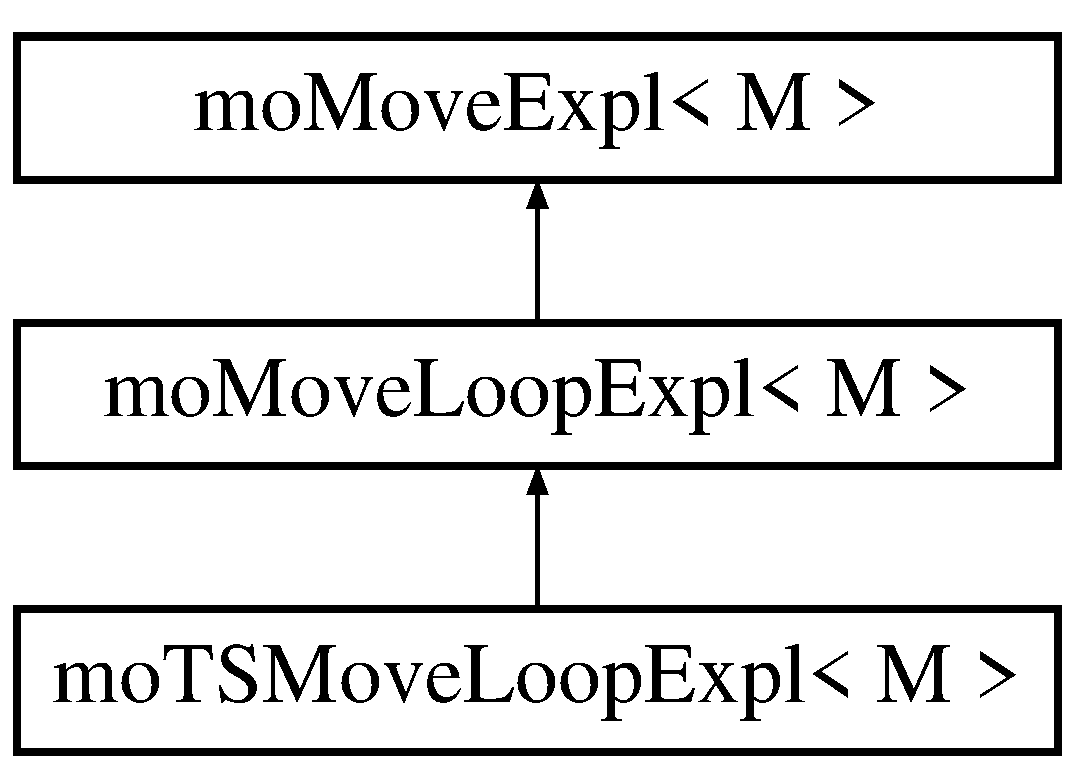
\includegraphics[height=5cm]{classmo_t_s_move_loop_expl}
\end{center}
\end{figure}
\subsection*{Public Member Functions}
\begin{CompactItemize}
\item 
\bf{mo\-TSMove\-Loop\-Expl} (\bf{mo\-Move\-Init}$<$ M $>$ \&\_\-move\_\-initializer, \bf{mo\-Next\-Move}$<$ M $>$ \&\_\-next\_\-move\_\-generator, \bf{mo\-Move\-Incr\-Eval}$<$ M $>$ \&\_\-incremental\_\-evaluation, \bf{mo\-Tabu\-List}$<$ M $>$ \&\_\-tabu\_\-list, \bf{mo\-Aspir\-Crit}$<$ M $>$ \&\_\-aspiration\_\-criterion)
\begin{CompactList}\small\item\em Constructor. \item\end{CompactList}\item 
void \bf{operator()} (const \bf{EOT} \&\_\-old\_\-solution, \bf{EOT} \&\_\-new\_\-solution)
\begin{CompactList}\small\item\em Procedure which lauches the exploration. \item\end{CompactList}\end{CompactItemize}
\subsection*{Private Types}
\begin{CompactItemize}
\item 
typedef M::EOType \bf{EOT}\label{classmo_t_s_move_loop_expl_47f42225e2ed096374b818bdb848a527}

\begin{CompactList}\small\item\em Alias for the type. \item\end{CompactList}\item 
typedef M::EOType::Fitness \bf{Fitness}\label{classmo_t_s_move_loop_expl_a1ba36c937b195ca2f7d1a24adaa7018}

\begin{CompactList}\small\item\em Alias for the fitness. \item\end{CompactList}\end{CompactItemize}
\subsection*{Private Attributes}
\begin{CompactItemize}
\item 
\bf{mo\-Move\-Init}$<$ M $>$ \& \bf{move\_\-initializer}\label{classmo_t_s_move_loop_expl_cd680d22382b9941d2c34133a641d443}

\begin{CompactList}\small\item\em Move initialisation. \item\end{CompactList}\item 
\bf{mo\-Next\-Move}$<$ M $>$ \& \bf{next\_\-move\_\-generator}\label{classmo_t_s_move_loop_expl_a2bbb593af2beefb05a307277c22b3d5}

\begin{CompactList}\small\item\em Neighborhood explorer. \item\end{CompactList}\item 
\bf{mo\-Move\-Incr\-Eval}$<$ M $>$ \& \bf{incremental\_\-evaluation}\label{classmo_t_s_move_loop_expl_491fa46e1cb7935cb515b27b85bf8765}

\begin{CompactList}\small\item\em Efficient evaluation. \item\end{CompactList}\item 
\bf{mo\-Best\-Impr\-Select}$<$ M $>$ \bf{move\_\-selection}\label{classmo_t_s_move_loop_expl_1caa6939fbe65ec4255e9e6dc3ce333b}

\begin{CompactList}\small\item\em Move selector. \item\end{CompactList}\item 
\bf{mo\-Tabu\-List}$<$ M $>$ \& \bf{tabu\_\-list}\label{classmo_t_s_move_loop_expl_0e5988a940ba218e87c53b7e56d79790}

\begin{CompactList}\small\item\em Tabu list. \item\end{CompactList}\item 
\bf{mo\-Aspir\-Crit}$<$ M $>$ \& \bf{aspiration\_\-criterion}\label{classmo_t_s_move_loop_expl_bdfc8efb22599c150b3c3d44cd416b09}

\begin{CompactList}\small\item\em Aspiration criterion. \item\end{CompactList}\end{CompactItemize}


\subsection{Detailed Description}
\subsubsection*{template$<$class M$>$ class mo\-TSMove\-Loop\-Expl$<$ M $>$}

Explorer for a Tabu Search algorithm. 

It is used by a \doxyref{mo\-TS}{p.}{classmo_t_s}. 



Definition at line 53 of file mo\-TSMove\-Loop\-Expl.h.

\subsection{Constructor \& Destructor Documentation}
\index{moTSMoveLoopExpl@{mo\-TSMove\-Loop\-Expl}!moTSMoveLoopExpl@{moTSMoveLoopExpl}}
\index{moTSMoveLoopExpl@{moTSMoveLoopExpl}!moTSMoveLoopExpl@{mo\-TSMove\-Loop\-Expl}}
\subsubsection{\setlength{\rightskip}{0pt plus 5cm}template$<$class M$>$ \bf{mo\-TSMove\-Loop\-Expl}$<$ M $>$::\bf{mo\-TSMove\-Loop\-Expl} (\bf{mo\-Move\-Init}$<$ M $>$ \& {\em \_\-move\_\-initializer}, \bf{mo\-Next\-Move}$<$ M $>$ \& {\em \_\-next\_\-move\_\-generator}, \bf{mo\-Move\-Incr\-Eval}$<$ M $>$ \& {\em \_\-incremental\_\-evaluation}, \bf{mo\-Tabu\-List}$<$ M $>$ \& {\em \_\-tabu\_\-list}, \bf{mo\-Aspir\-Crit}$<$ M $>$ \& {\em \_\-aspiration\_\-criterion})\hspace{0.3cm}{\tt  [inline]}}\label{classmo_t_s_move_loop_expl_be5cf0853777718c3bbcbef456b50bc7}


Constructor. 

\begin{Desc}
\item[Parameters:]
\begin{description}
\item[{\em \_\-move\_\-initializer}]The move initializer. \item[{\em \_\-next\_\-move\_\-generator}]The neighbourhood explorer. \item[{\em \_\-incremental\_\-evaluation}]A (generally) efficient evaluation. \item[{\em \_\-tabu\_\-list}]The tabu list. \item[{\em \_\-aspiration\_\-criterion}]An aspiration criterion. \end{description}
\end{Desc}


Definition at line 71 of file mo\-TSMove\-Loop\-Expl.h.

References mo\-TSMove\-Loop\-Expl$<$ M $>$::aspiration\_\-criterion, and mo\-TSMove\-Loop\-Expl$<$ M $>$::tabu\_\-list.

\subsection{Member Function Documentation}
\index{moTSMoveLoopExpl@{mo\-TSMove\-Loop\-Expl}!operator()@{operator()}}
\index{operator()@{operator()}!moTSMoveLoopExpl@{mo\-TSMove\-Loop\-Expl}}
\subsubsection{\setlength{\rightskip}{0pt plus 5cm}template$<$class M$>$ void \bf{mo\-TSMove\-Loop\-Expl}$<$ M $>$::operator() (const \bf{EOT} \& {\em \_\-old\_\-solution}, \bf{EOT} \& {\em \_\-new\_\-solution})\hspace{0.3cm}{\tt  [inline, virtual]}}\label{classmo_t_s_move_loop_expl_853743f2e21def3ea129556f47fafa55}


Procedure which lauches the exploration. 

The exploration continues while the chosen move is not in the tabu list or the aspiration criterion is true. If these 2 conditions are not true, the exploration stops if the move selector update function returns false.

\begin{Desc}
\item[Parameters:]
\begin{description}
\item[{\em \_\-old\_\-solution}]the initial solution \item[{\em \_\-new\_\-solution}]the new solution \end{description}
\end{Desc}


Implements \bf{eo\-BF$<$ const M::EOType \&, M::EOType \&, void $>$}.

Definition at line 90 of file mo\-TSMove\-Loop\-Expl.h.

References mo\-TSMove\-Loop\-Expl$<$ M $>$::aspiration\_\-criterion, mo\-TSMove\-Loop\-Expl$<$ M $>$::incremental\_\-evaluation, mo\-TSMove\-Loop\-Expl$<$ M $>$::move\_\-initializer, mo\-TSMove\-Loop\-Expl$<$ M $>$::move\_\-selection, mo\-TSMove\-Loop\-Expl$<$ M $>$::next\_\-move\_\-generator, and mo\-TSMove\-Loop\-Expl$<$ M $>$::tabu\_\-list.

The documentation for this class was generated from the following file:\begin{CompactItemize}
\item 
mo\-TSMove\-Loop\-Expl.h\end{CompactItemize}

\printindex
\end{document}
